\documentclass[12pt]{article}
\usepackage{verbatim}
\usepackage{lmodern}
\usepackage{graphicx}
\usepackage{color}
\usepackage{algorithm2e}
\usepackage{booktabs}
\usepackage{color}
\usepackage[table]{xcolor}
\usepackage{fancyhdr}
\usepackage[top=3cm, bottom=3cm, left=3cm, right=3cm]{geometry} 
\usepackage{hyperref}
\usepackage{url}
\usepackage{cite}
\usepackage{float}
\usepackage{listings}

\usepackage{array}


\hypersetup{colorlinks=true, linkcolor=black}
\pagestyle{fancy}
\renewcommand\arraystretch{1}
%\renewcommand\tabcolsep{3pt} 
\begin{document}

\lstset{language=C++,caption={Descriptive Caption Text},label=DescriptiveLabel,breaklines=true}


\title{ \bf{Navigation Stick for Visually Impaired using Ultrasonic Distance Sensors and WebCam}}
\date{}
\maketitle
\thispagestyle{empty}
\begin{center}
%\large \textbf{IIITB-OS-2011-5B}\\
\end{center}
\begin{center}
    \begin{tabular}[l]{ |l |l |l|l|}
    \rowcolor{gray!50} 
     \hline
    
    Name & Roll number & email-id & Contact Number\\ \hline \hline
    Divakar Ungatla & MT2010035 &divakar.ungatla@iiitb.org & 09535182022  \\ \hline 
    Hrishikesh Murali & MT2010048  &hrishikesh.murali@iiitb.org & 09591831139 \\ \hline 
    Nikhileshkumar Ikhar & MT2010049 & nikhileshkumar.ikhar@iiitb.org & 08197832897 \\ \hline 
    Joseph Jeffrey & MT2010057 & joseph.jeffrey@iiitb.org & 09194632897 \\ \hline 
    Julius Canute & MT2010058 & julius.canute@iiitb.org & 09535182022 \\ \hline


    \hline 
    \end{tabular}
\end{center}

\vfill
\begin{center}
\textbf{International Institute of Information Technology,Bangalore}
\textbf{www.iiitb.ac.in}
\end{center}

\newpage
\section*{Abstract}
This project aims at aiding a visually impaired person in navigating within an indoor environment. For this, we use a bot which will take his commands and act accordingly. The bot is in the form of a stick, with commands taken from a mouse. As he/she navigates within the environment, the bot learns the map and strives to achieve a full mapping of the environment around it, so that it can guide the person with the best of it's ability.\\\\
We use the SLAM algorithm to localize and map the environment. We use a BeagleBoard xM Rev C as the core processing unit for our bot, and ultrasonic sensors along with USB cameras to sense the environment. We have provided a full-fledged framework for the ultrasonic sensors, thus making it very easy for developers to futher develop this project using sensors. We give auditary feedback to the visually impaired person. This feedback tells the person about his/her location derived from SLAM.

\newpage
\section*{Acknowledgements}
We would like to express our deep-felt gratitude to our guide Prof. Poonacha P. G., International Institute of Information Technology, Bangalore, for his advice, encouragement, enduring patience and constant support. He has always provided us with clear explanations when we were lost, constantly driving us with energy, giving us their valuable time. We are indebted to him for the unparallel support that he has lent to make this project a huge success.\\\\
Hrishikesh Murali\\
Julius Canute\\
Joseph Jeffrey\\
Nihilesh Kumar Ikhar \\
Divakar Ungatla\\

\newpage
\tableofcontents

\newpage
\section{Introduction}
		
     The objective of the project is to design a stick equipped with distance measuring ultrasonic sensors and webcam which helps in detecting obstacles and alerting the blind person. A localization algorithm is also used to detect the position of the blind person in an indoor environment.\\

The blind navigation device has been implemented using a Beagle Board xM Rev C as the source for the stick's intelligence. Ubuntu Linux has been installed on the board, which runs a 3.0.4 version of the Linux kernel. The stick is aided by a bot at its bottom for better navigation.
A slightly modified SLAM algorithm is used for localization. The readings of the Ultrasonic sensors and images from the webcam are used for obstacle detection.\\

The remainder of the paper is organised as follows: Section2 explains the interfacing of the UV sensors to the beagle board and the code that is deployed on the board in order to collect and analyse the information from the sensors. It also describes the interfacing between the beagle board and the bot. Section3 explains the localization algorithm used and simulation results for the same. Section4 deals with the image interpretation techniques used for obstacle detection using the webcam. Section5 draws a conclusion and provides guidelines for future work.\\

\section{Ultrasonic sensor interfacing with beagle board}
The blind navigation device has been implemented using a BeagleBoard xM Rev C as the source for the stick's intelligence. Ubuntu Linux has been installed on the board, which runs a 3.0.4 version of the linux kernel. Interaction between the board and the wheels happen through the expansion header of the beagleboard, which contains the GPIO pins. We use input from eight ultrasonic sensors, which are connected to the beagleboard via the Universal Serial Bus (USB). We have two USB hubs, which multiplex four ultrasonic sensors each. So in essence, we use just two physical USB ports of the beagleboard. These ultrasonic sensors use the serial protocol for communication, so we have to have a "Serial port to USB" convertor, and connect it to the hub. This eliminates the need of us having to follow the serial protocol in user-space programs.
\\
\\
We have a USB mouse connected to the beagleboard, which is the main source of input from the user. The mouse has three buttons - left, right and center. We follow the following configuration for input:
\\
\\
\\
\begin{itemize}
\item Left - Turn the device left.
\item Right - Turn the device right.
\item Center - Toggle starting the device.
\end{itemize}
If the person handling the device chooses to start the device, he or she has to press the center mouse button. If he wishes to stop it, he or she as to press the center button again. If he or she chooses to turn left, then the user has to press the left mouse button. The
device then turns left. It continues to turn left till the user chooses to press the center button again. Then it will move straight. A similar logic works for turning to the right too.
\\
\\
The beagleboard runs a user-space program written in the C language, which takes input from the ultrasonic sensors and processes it. It also takes a If any of the ultrasonic sensors detect that an obstacle is too near, then the programs stops the motors from running and provides a voice output to the person handling the device. The voice output tells the person how far the obstacle is. Then, the program waits for input from a user, whether to turn left or right. If left, then the device turns till the user chooses to press the center mouse button. A similar argument holds true for moving right too.
\begin{center} 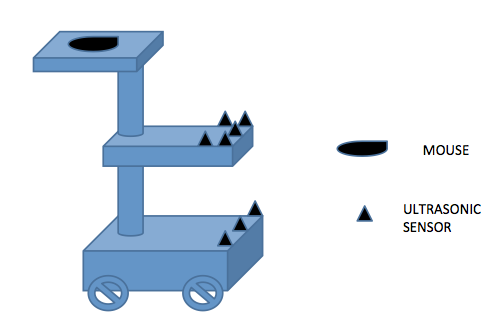
\includegraphics[scale=0.4]{bot} \end{center}
There exists a driver circuit for each motor. Since there are four wheels, we have four motors and hence four driver circuits. These driver circuits can run on a 5V supply, which can be given from the beagleboard's expansion header. These driver circuits also provide two leads each, which can be configured to run the motors. The driver circuit runs the motor based on the potential difference between these two leads. They work based on an XOR logic. Supposing A and B are the two leads of the driver circuit:
\begin{center} 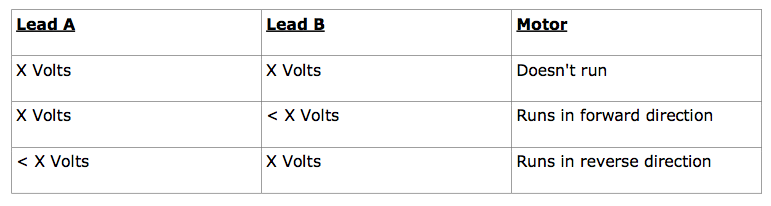
\includegraphics[scale=0.4]{table1} \end{center}
The value X depends on the Vcc supply given to the driver circuit. We have seen that for a Vcc supply of 5V, the value of X is 3.1V.
An interface for the ultrasonic sensors has been provided in the program itself. Now, all a developer needs to do is specify the ultrasonic sensors' configuration in a configuration file. Each ultrasonic sensor in the configuration file must have the following details:
\\
\\
\begin{verbatim}
ultrasonic_sensor = {
sensor_device_name = /dev/ttyUSB2 
sensor_device_name = front_left_sensor 
data_format = feet
threshold_distance = 3
datasize = 5
datastart_offset = 1
priority = 0
}
\end{verbatim}
This means that the ultrasonic sensor exists as a character device named "/dev/ttyUSB2" of the linux system. The data representation for this sensor is in feet, and the threshold distance is 3 feet. Priorities can be set for sensors, and the program appropriately prioritizes each sensor. The rest of the fields - datasize, datastart$\_$offset have been given so that this interface can be used with any type of sensor, where we just have to specify at which byte offset the data starts, and what is the number of bytes that have to be read from the device.

\begin{verbatim}
register_sensor ( struct ultrasonic_sensor *sensor );
\end{verbatim}
\begin{itemize}
\item This function allocates memory for the sensor - registers it with the program.
\end{itemize}

\begin{verbatim}
deregister_sensor ( struct ultrasonic_sensor *sensor );
\end{verbatim}

\begin{itemize}
\item This function deallocates the memory allocated for the sensor and removes
the sensor's association from the program.
\end{itemize}

\begin{verbatim}
start_sensor ( struct ultrasonic_sensor *sensor );\end{verbatim}
\begin{itemize}
\item This function starts taking input from an ultrasonic sensor - comparing the input with a threshold value and calling an 'alert' function which gives voice output to the user.
\end{itemize}

\begin{verbatim}
start_sensor ( struct ultrasonic_sensor *sensor );\end{verbatim}
\begin{itemize}
\item This function starts taking input from an ultrasonic sensor - comparing the input with a threshold value and calling an 'alert' function which gives voice output to the user.
\end{itemize}

\begin{verbatim}
stop_sensor ( struct ultrasonic_sensor *sensor );\end{verbatim}
\begin{itemize}
\item This function stops taking input from the specified ultrasonic sensor.
\end{itemize}

\begin{verbatim}
read_data_from_sensor ( struct ultrasonic_sensor *sensor, int format );\end{verbatim}
\begin{itemize}
\item This function reads data from the sensor, and returns the appropriate value in the format specified.
\end{itemize}

\begin{verbatim}
alert ( struct ultrasonic sensor *sensor, float distance );\end{verbatim}
\begin{itemize}
\item This function sends an analog voice output to the user, saying "Wait! Obstacle at X inches/feet/cm/m". The value 'X' is the second argument 'distance' and the format is specified in the first argument structure 'sensor'.
\end{itemize}
The program being run on the beagleboard is an ELF32 executable, which does the following:
\begin{itemize}
\item Initializes the wheel I/O. It configures the GPIO pins of the expansion headeras output pins.
\item Reads the configuration file, thus registering all ultrasonic sensors with the program.
\item Creates a thread, which will monitor input through the USB mouse.
\item Spawns multiple threads,once for each ultrasonic sensor - will monitor it, and appropriately alert the user if an obstacle is within the threshold distance.
\item If the user presses the center mouse button, then it calls the "toggle$\_$start" function, which will start the device.
\item The device continues going straight till an input is given from the mouse by the user, or if the device detects that an obstacle is too close.
\item If the user presses the left/right mouse button, it moves left/right respectively, until the user presses the center mouse button again.
\item If an obstacle is detected to be too close to the device, the program immediately stops the device by calling the "stop$\_$device" function, which will stop the wheels.
\item It waits for input from the user again.
\item This continues till the user manually stops the device by pressing the center mouse button.
\end{itemize}
A rough layout of the device interaction with the wheel's driver circuit is shown below:
\\
\begin{center} 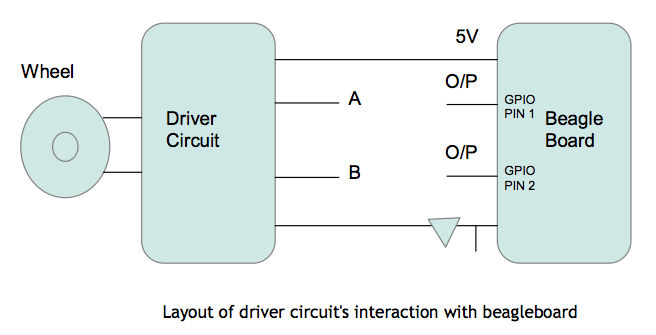
\includegraphics[scale=0.4]{driver_circuit} \end{center}
A USB camera is to be interfaced with the beagleboard. We have confirmed that the USB camera works with the beagleboard, and have also taken sample pictures to test it out. We are yet to integrate the image recognition code with the main program.
\section{Localization Using SLAM}
In the stick for visually impaired which we were developing for indoor environments, there was a need to identify the position of the blind person\cite{slam}. Given we have limited sensors to get information about the environment like we had 5 ultrasonic sensors and the approximate information given by the stick itself about its position and orientation. We needed a rough estimation of the person's position within the indoor environment, for which are surveys indicated to do localization.\\
\\
Localization is a mechanism by which a bot identifies where it is located within an environment based upon the information it has gathered from the environment. In this context there are different ways in which we can do this localization. One is feed the map to the bot so that it uses the map as well as the features it observes from the environment to mark its position within the supplied map\cite{slamm}. The map for instance can be represented in 2D or 3D. In other form of localization the bot dynamically constructs the map as it observes in the environment and mark its position based upon the constructed map, this approach is called SLAM (Simultaneous localization and Mapping).\\
\\
We thought that the first approach might not be scalable as it requires to feed in the map every time the bot is placed in the new environment, So we chose the latter on in which map is constructed dynamically. In the latter approach we implement a variation of SLAM using the limited sensor information we have. In this approach we extract a set of landmarks\cite{landmark} from the environment and use that as a reference to identify the position of the bot relative to the landmarks. A landmark in our case can be thought of as a point in 2-Dimension.\\
\\
\subsection{Algorithm}
To roughly estimate the position of the bot in the environment we use Extended Kalman Filter. Estimation process can be broadly divided into three step process.
\begin{itemize}
\item Use the odometry reading given by the bot and the position of the landmarks to roughly approximate the bots position.
\item As the odometry is prone to error we use the sensor information to identify the position of the bot. Depending on the level to which we trust the odometry and sensor performance we update the bots position.
\item If there are any unobserved landmarks during the process of estimation it is added to the set of observed landmarks and will be used in the computation of positoin there after wards.
\end{itemize}
\begin{center} 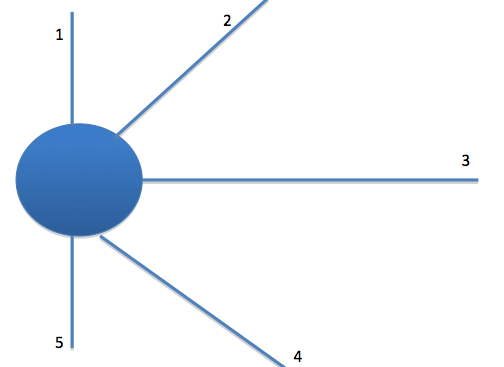
\includegraphics[scale=0.4]{sensor} \end{center}
\subsection{Model of the Stick}
The above figure indicates the way in which ultrasonic sensors are placed around the stick. Starting from the left of the stick (sensor1) each sensor is placed at 45 degree angle from each other. Everytime when the distance is measurement is required from the bot, we query the distance the bot has moved since our last invocation, which inturn can approximately be calculated by the span of time in which the bot is in movement and the distance the bot moved in 1 sec(which has to experimentally set based upon the load on the stick). The angle stick has turned has to be calculated in a similar way like the angle which the bot turned in 1 sec times the time bot spent in sideway movement.
\subsection{Landmark Extraction}
Given the model of the bot we extract landmarks based upon the direct sensor information we get from the ultrasonic sensors and we assign sensor numbers on which the reading has been taken.\\
\begin{center} 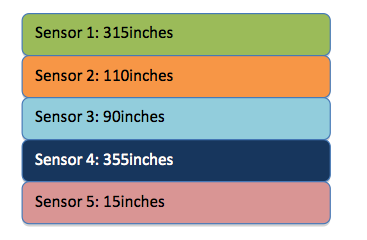
\includegraphics[scale=0.4]{pic1} \end{center}
We only compare extracted landmark\cite{landmark} info from a sensor with the landmark info taken by the same sensor. For example if there are previously extracted landmarks of sensor 5 and sensor 5 gives a new reading based upon its new position, we compare sensor 5 information with the information sensor 5 has previously stored about the landmark\cite{sonar}.\\
\\
We assume the landmark to be reobserved if the new landmark observed by the sensor is within a radius 'R' which can be experimentally computed and set.\\
\\

We can convert a landmark to a cartesian coordinate using the following procedure.\\
\\
\begin{center} 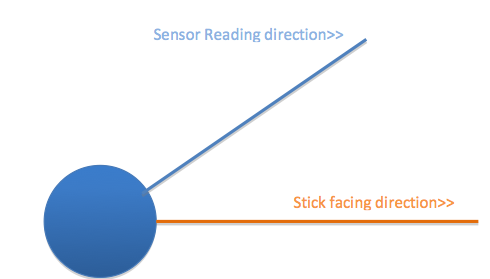
\includegraphics[scale=0.4]{pic2} \end{center}
Let Rx and Ry be the stick position, R be the range reading observed from the sensor, be the stick positoin and be the relative angle in which the sensor is placed relative to the stick orientation, it can be either positive or negative. Hence the landmark position Lx and Ly are calculated using the following formula:\\
\begin{center} 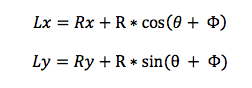
\includegraphics[scale=0.4]{pic3} \end{center}


\subsection{Terminologies}
Let X be the state vector of the stick represented as:\\
\\
\begin{center} 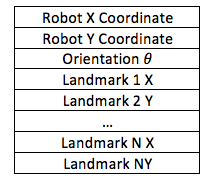
\includegraphics[scale=0.4]{t1} \end{center}
Let P be the covariance matrix\cite{kalman} represented as:\\
\\
\begin{center} 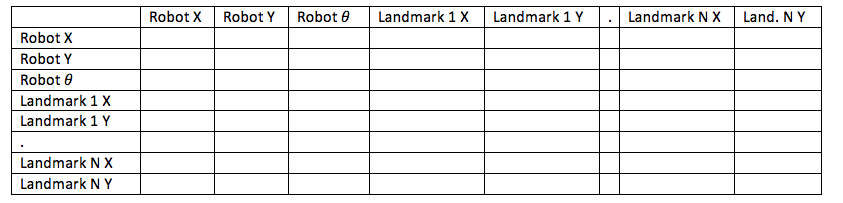
\includegraphics[scale=0.4]{t2} \end{center}
P maintains the covariance between Robot-Robot,Robot-Landmark,Landmark-Landmark positions.
Let Q be:\\
\begin{center} 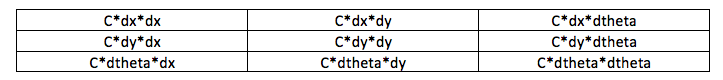
\includegraphics[scale=0.4]{t4} \end{center}
Q is updated to reflect the error in the control and its factor of implication to its orientation and position, dx, dy represents the distance the bot has progressed along the x and y direction since the last measurement, dtheta represents the change in orientation since the last measurement.\\
\\
Let A be:\\
\begin{center} 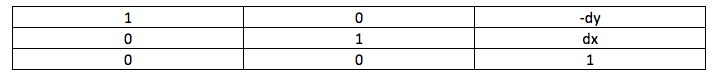
\includegraphics[scale=0.4]{t5} \end{center}
A represents the jacobian of the prediction model which is use to linearise the function so it can be used in Kalman filter in computation of Kalman gain\cite{filter}.\\
\\
Range and bearing is calculated as follows:
\begin{center} 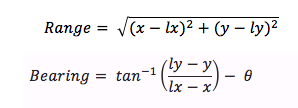
\includegraphics[scale=0.4]{t6} \end{center}
Here x,y, are the bots position and orientation, lx, ly are the observed landmarks x and y. Let H be:\\
\begin{center} 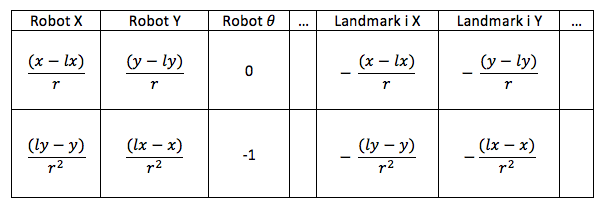
\includegraphics[scale=0.4]{t7} \end{center}
Say if we are currently observing the Ith landmark then H is initialized with the value as shown for the Ith landmark alone other landmarks are initialized with zero. H will be used in computation of Kalman gain.\\
\\
Let R be:\\
\\
\begin{center} 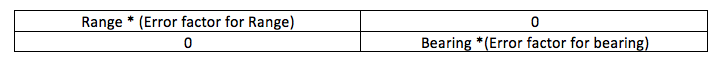
\includegraphics[scale=0.4]{t8} \end{center}
Let JXR be Jacobian of the prediction model for predicting landmarks based on robot position be represented by:\\
\\
\begin{center} 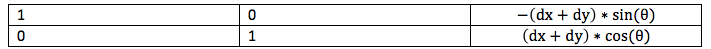
\includegraphics[scale=0.4]{t9} \end{center}
Let JZ be Jacobian of the prediction model for predicting landmarks based on range and bearing:\begin{center} 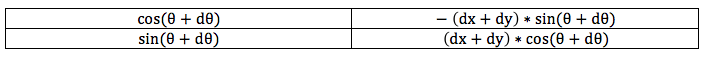
\includegraphics[scale=0.4]{t10} \end{center}
\subsection{Computation of Parameters}
\begin{center} 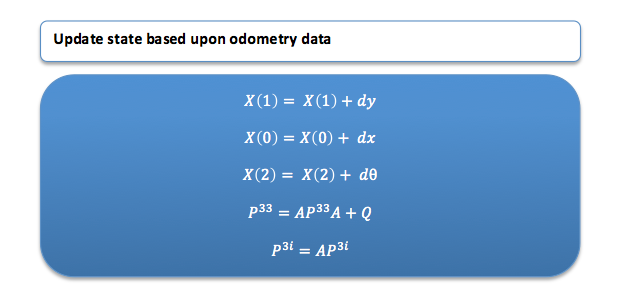
\includegraphics[scale=0.4]{p1} \end{center}
\begin{center} 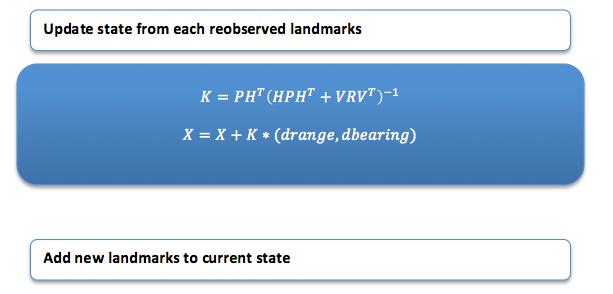
\includegraphics[scale=0.4]{p2} \end{center}
\begin{center} 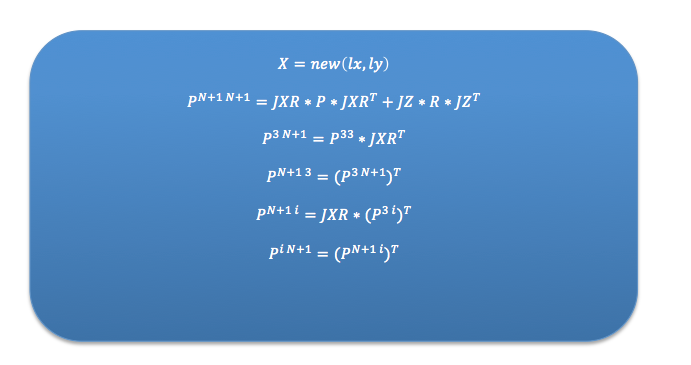
\includegraphics[scale=0.4]{p3} \end{center}
\subsection{Final Remarks}
\begin{center} 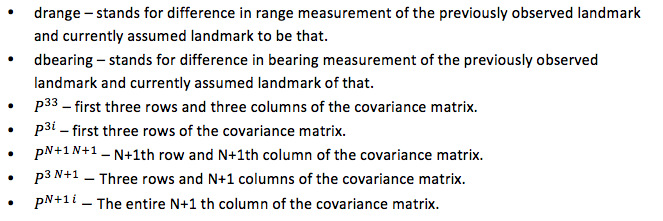
\includegraphics[scale=0.4]{p4} \end{center}
\subsection{Implementation}
Currently the localization is tested in the simulation environment.
For this a simulation model was developed to simulate odometed and sensor reading:
\\
\\
\begin{center} 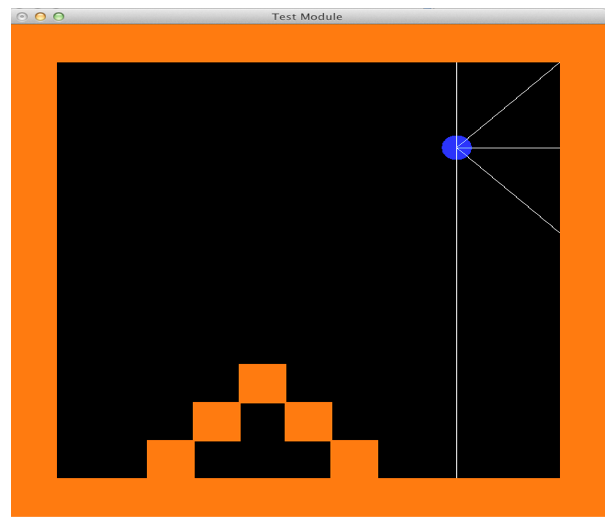
\includegraphics[scale=0.4]{p5} \end{center}

The simulation model shows stick as a blue color circle, the walls are shown in orange color. The sonar rays are shown emanating in white color. The sonar rays gives distance measurement in range of 0 to 2. The arrow keys can be used to drive the stick as of now.The map can be dynamically created by editing a binary 2D array which represents an obstacle at [i][j] if map[i][j] is set to 1 and 0 otherwise\cite{glut}.
\begin{center} 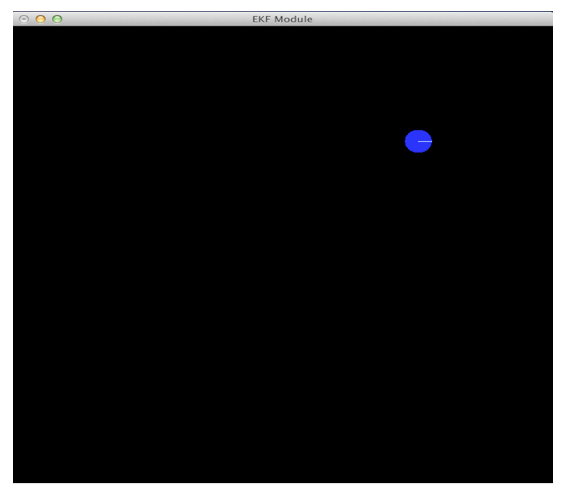
\includegraphics[scale=0.4]{p6} \end{center}

The localization module is connected to the simulation model via socket. The simulation model sends the readings it observer from the environment to localization module and the localization module tries to map out the environment.
\begin{center} 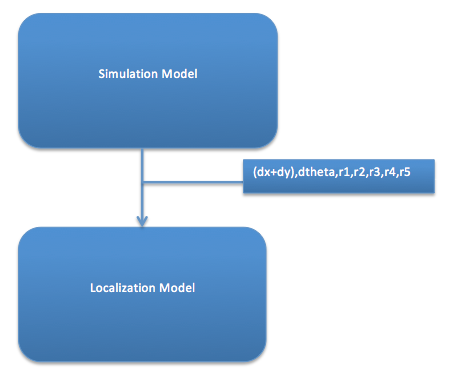
\includegraphics[scale=0.4]{p7} \end{center}

The simulation model sends information about distance the stick has moved since last measurement(dx+dy). The orientation the stick has turned since last measurement dtheta and range readings r1,r2,r3 r4, r5 respectively. The simulation model can easily be decoupled and interfaced with the actual bot by scaling the sensor readings in a scale of 0 to 2.

\subsection{Test Results}
\begin{center} 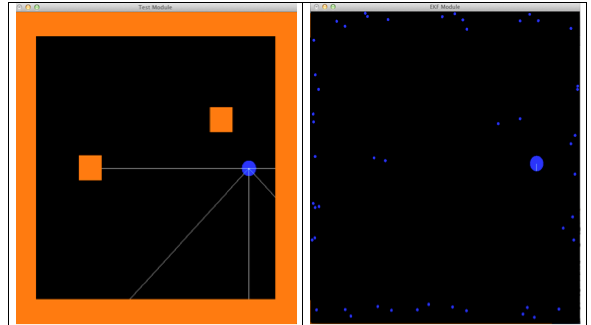
\includegraphics[scale=0.4]{p8} \end{center}
\begin{center} 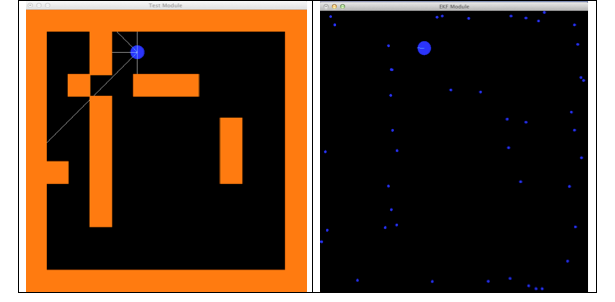
\includegraphics[scale=0.4]{p9} \end{center}

The blue dots in diagram represents the extracted landmark. The algorithm was tested by setting the average distance observed as 0.5 given that the screen coordinate span form (-1,-1) to (1,1)\cite{boost}.

\subsection{Suggestion and Conclusion}
There are a few suggestions in terms of extending this algorithm.
\begin{itemize}
\item The algorithm right now does not have a hard stop to detect the completion of landmark extraction, identifying when to stop the algorithm from extracting landmarks is a challenging problem.
\item There is a problem of closing the loop that has to be addressed. Where a bot starts and reaches the same position in some other way.
\item There is a problem of map construction of the envrionment which inturn requires sophisticated operations in using the camera and doing a scan(swipe 180).
\item The algorithm also can be extended to incorparate data with a specific set of landmarks which inturn can be used to give auditory output to the blind person regarding his current position.
\end{itemize}

\section{Object Detection}
\subsection{Litreature Study}
The Blind navigation system requires feedback from sensors to look find the path. These sensors are ultra sonic sensors and camera.\\
\\
Robot is guided without human intervention. It has to find its path between obstacles. Our robot uses eight ultra-sonic sensors to find the obstacles and a camera. Camera gives the output as image frame. Continuous image frame is processed to tell object in ahead of robot.\\
\\
Generally there are two main objective associated with images. One, object detection and second object recognition.\\
\\
Object detection means to find any object of interest in image. It can be finding any human, box, table etc. In any image, to find presence of a particular object is object recognition. For e.g. finding presence of human face, box, pen in an image. Both require finding the object based on some features.\\
\\
In our case we need to find the presence of object it can be any object. Right now, we are not interested in finding the type of object (detection). After determining the position of object we can guide the robot to inform user about object or robot can use this information to move around object without touching it.\\
\\
We considered various algorithms for object recognition like SIFT (Wikipedia), Haar wavelet responses (Gary Bradski, 2008). Both this methods requires training with images to create object feature database. For SIFT it requires around 200 positive images. Positive image have object inside the image. For Haar wavelet, it requires more than 2000 positive and negative images. Negative image don't have object inside it. Also, both the methods require training for different set of objects. In other word to detect box shaped object, we have to extract feature with using 200 images. If we want to detect chair, we need another set of 200 images for feature extraction. This is very cumbersome process. In case of Haar wavelet, this task is very huge. Also these methods don't serve the purpose. We have to find the object in path of robot. Right now we ignore the need to recognize the object.\\
\\

\subsection{Design Plan $\&$ Flow}
We assume the following things. These assumptions are needed to maintain consistency over repeated number of experiments.\\
\\
Camera on robot is always pointing towards the floor/ground. We assume most are of floor is free, unoccupied with other objects. Object is made of non-reflective surface. Object has colour different than floor colour. Also we assume floor is made of one colour. We can consider floor as background and object present on floor as foreground. First we have to detect the floor and then we can detect object in it. So we have to separate foreground and background. We are using OpenCV library (Gary Bradski, 2008). It is used for image processing operation in real time. It provides API's for various operation.\\
\\
\subsection{Contour Based Object Detection}
First approach was to separate background and foreground using contours. Contours are region in which each pixel have same characteristics or can have computed property like colour, intensity, texture. OpenCV is used to find contour in an image. Before giving image to find the contour we need to spread out the pixel information in neighbouring pixel else, each pixel can act as a contour. We used image pyramid. In real world they are used multi-scale image representation. It involves two methods Gaussian Pyramid and Laplacian Pyramid. Gaussian pyramid is used to get down sampled image. Image is first smoothened with filter and then down sampled. This results in loss of information. Laplacian pyramid are used to restore the image but, restored image is not original image. Resultant image after these operations is segmented image.
\\
\\
\begin{center} 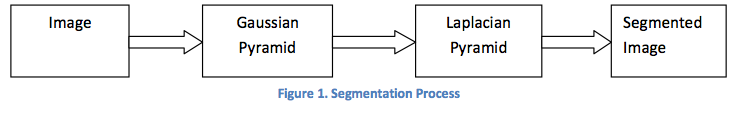
\includegraphics[scale=0.4]{a1} \end{center}

This segmented image is given to find contour. We access the each contour one by one and calculate its associated area. We store the largest contour. This is our background or floor. Because floor is supposed to be relatively free from object. We did this but results were not satisfactory. A large part of contour was changing with slight change is light condition.\\
\\
\\
\begin{center} 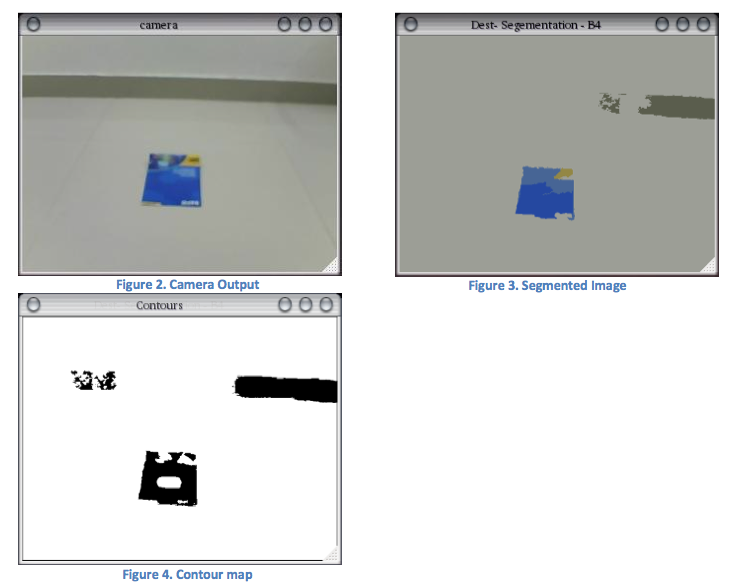
\includegraphics[scale=0.4]{a2} \end{center}
Figure 2 is segmented image. Level of segmentation can be changed in code. In Figure 3, white region shows area inside the contour.\\
\\
\subsection{Colour Based Object Detection}
In next method we uses colour information present in image. The image is first converted in HSV (Hue, Saturation, and Value) format (Wikipedia). Hue represents type of colour. Saturation represents the concentration of colour and Value represents brightness. First we fill a range of same colour with one and only one colour. For following strip of red colour is filled with red colour with HSV value (0, 255, and 255)\cite{hslhsv}.\\
\\
\begin{center} 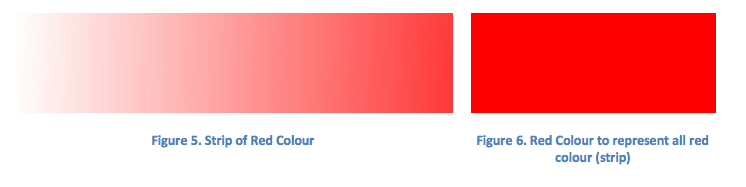
\includegraphics[scale=0.4]{a3} \end{center}
We have decided to divide whole colour range in eleven parts namely black, white, gray, red, orange, yellow, green, aqua, blue, purple, and pink. We go to each pixel and map it in one of eleven colours. Then we fill that pixel with corresponding one of the eleven

colours. We keep the track of count of no of pixel mapped to each colour. Then we calculate percentage of all colours in image. The colour with max value is representing our background.\\
\\
We divide whole image in blocks of 10x10 or 20x20 etc. Then in each block we find colour percentage for each of eleven colours. If colour percentage of any one colour in block other than background colour is greater than threshold, we say it as presence of object in that block. In the end we find the position of objects in image and tell user if object is present at left, middle or right side in front direction.\\
\\
\subsection{Installation of OpenCV libraries on Beagle board}
We have installed Ubuntu 11.04 on Beagle board. To install OpenCV\cite{opencv} libraries follow following steps
\begin{itemize}
\item Connect Beagle board to internet.
\item Run $<$ sudo apt-get update $>$
\item Run $<$ apt-cache search cv $>$, it will show names of computer vision libraries.
\item Install them all, using $<$ sudo apt-get install pkg-name $>$
\end{itemize}

\subsection{Compiling and running code}
Program is written in 'C' language. Go to folder where code is kept.
\begin{itemize}
\item Download the source code using $<$ svn checkout http://nab- iiitb.googlecode.com/svn/trunk/ nab-iiitb-read-only $>$
\item Compile it using $<$ gcc -L/usr/lib -o "NAB" -lcvaux -lhighgui -lcv ColorObject.c $>$
\item Run the program using $<$ ./NAB x $>$. Where x is USB port at which camera is connected.
\end{itemize}

\subsection{Experimental Setup}
Our robot setup has camera fitted at height of approx 35 cm. The camera angle is adjusted such that is min distance camera can look is 35 cm. We put six A4 size sheets on floor and took image of it.\\
\\
\begin{center} 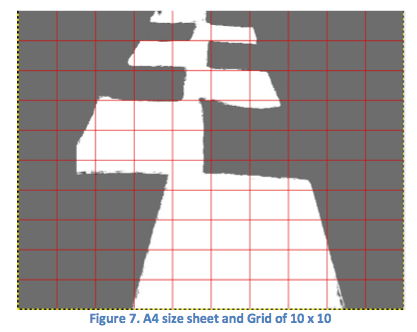
\includegraphics[scale=0.4]{a4} \end{center}
We see first A4 size sheet looks bigger than last sheet. For processing we are dividing the images in block. First A4 sheets fits in approx 4.5 blocks and farthest block contains two sheets. This is perspective problem. We manually measured the block distance. In Figure 7, first block value is 7cm. Hence any object falling in block 1 is at
distance, 45 +7 = 42cm.\\
\\
\begin{center} 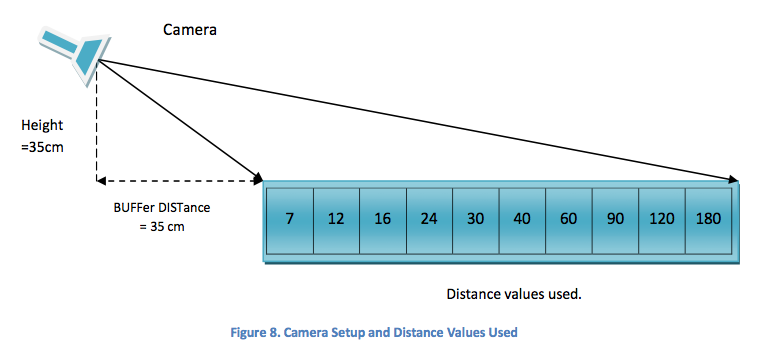
\includegraphics[scale=0.4]{a5} \end{center}
\subsection{Results}
The following picture shows both conditions, with and without object. Our object is small notebook blue in colour. In first pictures object is absent. So the resultant block array contains all zeros. In next picture object is present in middle of frame. Corresponding to object position, 3 block contains 1 other contain zero. The object distance is, 35 + 40 = 75cm.
\begin{center} 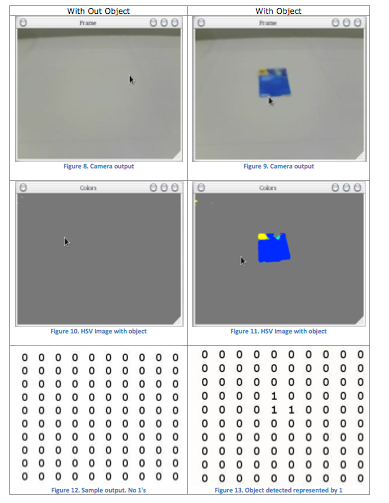
\includegraphics[scale=0.4]{a6} \end{center}
\subsection{Suggestion $\&$ Conclusion}
The camera is looking at object at slanted angle. This gives rise to perspective distortion. This needs to be corrected. This algorithm is very sensitive to changes in light conditions. It should be removed.\\
\\
This setup can be effectively used to detect objects at smaller distance.\\
\\
\subsection{Conclusion and Future Work}
The Ultrasonic sensors had been successfully interfaced with the Beagle board. Interfacing the beagle board with the bot is currently going on. The localization algorithm had been simulated and tested. It should be deployed on the actual system. The areas where the localization algorithm can be improved are mentioned in the suggestions section of section3.

\bibliographystyle{IEEEtran}
\bibliography{citation}

\newpage
\section{Appendix A - Device driver source}
\begin{lstlisting}[caption="Main Program - Starts the device"]
/* 
 * Author: Hrishikesh Murali 
 * Date:   4th November, 2011
 * Copyright 2011 NAB. All rights reserved.
 */ 
#include <stdio.h> 
#include <stdlib.h> 
#include <string.h> 
#include <unistd.h> 
#include <pthread.h> 
#include <fcntl.h> 
#include "obstacledetect.h" 
#include "device.h" 

int num_threads = 0; 

extern char mousefilename[]; 

/* Tell the user as to how (s)he must use the program! */ 
void usage ( char *progname ) { 
	printf ( "Usage: %s <path_to_config_file>\n", progname ); 
	return; 
} 

void* monitor_mouse_event ( void *argument ) { 
	while ( TRUE ) { 
		int command = get_mouse_command(); 
		if ( command == TOGGLE_START ) { 
			toggle_start(); 
		} 
		else if ( command == TURN_LEFT ) { 
			turn_left(); 
		} 
		else if ( command == TURN_RIGHT ) { 
			turn_right(); 
		} 
		usleep ( 1000 ); 
	} 
} 

/* This function is used by each thread which is spawned. 
 * It opens the device, and reads from it signals an alarm 
 * if the nearest obstacle is less than a certain threshold. 
 */ 
void* monitor_sensor ( void *argument ) { 
	ultrasonic_sensor *sensor = (ultrasonic_sensor*) argument; 

	/* Open the device */ 
	if ( start_sensor ( sensor ) != SUCCESS ) { 
		printf ( "Failed to open device %s in read-only mode, check if device exists and permissions are set!\n", sensor->device_name ); 
		goto exit; 
	} 

	float distance = INVALID; 

	/* Do this all the time! */ 
	while ( TRUE ) { 
		/* Read the data from the sensor */ 
		distance = read_data_from_sensor ( sensor ); 
		 
		if ( distance == INVALID ) { 
			if ( stop_sensor ( sensor ) != SUCCESS ) { 
				printf ( "Couldn't stop sensor!\n" ); 
				fflush ( stdout ); 
			} 
			goto exit; 
		} 
		 
		if ( distance < sensor->threshold_distance ) { 
			/* Oops, obstacle too near! Signal an alarm!! */ 
			alert ( sensor, distance ); 
		} 
		usleep(1000); 
	} 

exit: 
	num_threads--; 
	return NULL; 
} 

int initdevice ( char *configfile, int *number_of_sensors, ultrasonic_sensor **sensors, pthread_t *monitor_mouse_event_thread ) { 

	init_wheelio (); 
	*sensors = register_sensors ( configfile, number_of_sensors ); 
	 
	if ( number_of_sensors <= 0 || sensors == NULL ) { 
		if ( number_of_sensors <= 0 ) { 
			printf ( "No sensors provided!\n" ); 
		} 
		if ( sensors == NULL ) { 
			printf ( "Couldn't read from config file %s!\n", configfile ); 
		} 
		return FAILURE; 
	} 
	pthread_create ( monitor_mouse_event_thread, NULL, monitor_mouse_event, NULL ); 
	return SUCCESS; 
} 

/* This is the main function - calls the necessary functions */ 
int main ( int argc, char **argv ) { 

	if ( argc == 1 ) { 
		/* Tell the user how to execute the program */ 
		usage(argv[0]); 
		return FAILURE; 
	} 
	int number_of_sensors = 0; 
	ultrasonic_sensor *sensors = NULL; 
	pthread_t monitor_mouse_event_thread; 
	if ( initdevice ( argv[1], &number_of_sensors, &sensors, &monitor_mouse_event_thread ) != SUCCESS ) { 
		printf ( "Couldn't initialize the device!\n" ); 
		return FAILURE; 
	} 
	 
	/* Create an array of threads */ 
	pthread_t *monitor_thread; 
	monitor_thread = (pthread_t*) malloc ( sizeof(pthread_t) * number_of_sensors ); 

	/* Spawn as many threads as specified. */ 
	int sensor_num = 0, retval = INVALID; 
	for ( sensor_num = 0; sensor_num < number_of_sensors; sensor_num++ ) { 
		retval = pthread_create ( &monitor_thread[sensor_num], NULL, monitor_sensor, (void*) &sensors[sensor_num] ); 
		if ( retval != SUCCESS ) { 
			/* For some reason, the thread couldn't be created. Not enough resources? */ 
			printf ( "Failed to create thread number %d for device %s - ERROR %d", sensor_num+1, sensors[sensor_num].device_name , retval ); 
			goto exit; 
		} 
	} 

	num_threads += number_of_sensors; 
	while ( num_threads ) { 
		/* Wait till all the threads have finished executing and have exited. 
		 * It's not good to infinitely wait as it'll eat up one whole processor, 
		 * so sleep for 1 millisecond and check again. 
		 */ 
		sleep(1); 
	} 
exit: 
	if ( deregister_sensors ( &sensors, number_of_sensors ) != SUCCESS ) { 
		printf ( "Couldn't deregister all sensors!\n" ); 
	} 
	deinit_wheelio (); 
	free ( monitor_thread ); 
	return SUCCESS; 
}
\end{lstlisting}
\begin{lstlisting}[caption="device.h - Device related headers"]
/* 
 * Author: Hrishikesh Murali 
 * Date:   4th November, 2011 
 * Copyright 2011 NAB. All rights reserved.
 */ 
#define SUCCESS 0 
#define FAILURE 1 
#define INVALID -1 
#define TRUE 1 
#define FALSE 0 
#define BOOL int 
#define BYTE char 

#define STOPPED 0 
#define RUNNING 1 
#define TURNING 2 
#define NUM_WHEELS 4 
#define MOUSE_DATASIZE 8 
#define TOGGLE_START 1 
#define TURN_LEFT 2 
#define TURN_RIGHT 3 

#define STOP 0 
#define MOVE_FORWARD 1 
#define MOVE_REVERSE 2 

void init_wheelio ( void ); 
void deinit_wheelio ( void ); 
int get_mouse_command ( void ); 
int toggle_start ( void ); 
void turn_left ( void ); 
void turn_right ( void );
\end{lstlisting}
\begin{lstlisting}[caption="device.c - Device related source"]
/* 
 * Author: Hrishikesh Murali 
 * Date:   4th November, 2011 
 * Copyright 2011 NAB. All rights reserved.
 */ 
#include <stdio.h> 
#include <string.h> 
#include <fcntl.h> 
#include <stdlib.h> 
#include <unistd.h> 
#include <errno.h> 
#include <pthread.h> 
#include "device.h" 

int mousefd = INVALID; 
int device_state = STOPPED; 

static char mousefilename[] = "/dev/hidraw0"; 

/* 
	Wheel1 -------------- Wheel2 
		|           |
		|           | 
		|           | 
		|           | 
		|           | 
		|           | 
		|           | 
	Wheel3 -------------- Wheel4 

	wheels[] = { Wheel1, Wheel2, Wheel3, Wheel4 }; 

*/ 

int wheels_pins[NUM_WHEELS][2] = { {140, 142}, {139, 138}, {156, 157}, {131, 130} }; 
int wheels[NUM_WHEELS] = { STOP, STOP, STOP, STOP }; 
pthread_mutex_t wheel_mutex = PTHREAD_MUTEX_INITIALIZER; 

/* These functions assume that the caller has 
 * previously acquired the lock for the wheels 
 */ 
static inline void move_forward ( int wheel_number ) { 
	char command[100]; 
	sprintf ( &command[0], "echo \"1\" > /sys/class/gpio/gpio%d/value", wheels_pins[wheel_number-1][0] ); 
	system ( command ); 
	sprintf ( &command[0], "echo \"0\" > /sys/class/gpio/gpio%d/value", wheels_pins[wheel_number-1][1] ); 
	system ( command ); 
	wheels[wheel_number-1] = MOVE_FORWARD; 
} 

static inline void move_reverse ( int wheel_number ) { 
	char command[100]; 
	sprintf ( &command[0], "echo \"0\" > /sys/class/gpio/gpio%d/value", wheels_pins[wheel_number-1][0] ); 
	system ( command ); 
	sprintf ( &command[0], "echo \"1\" > /sys/class/gpio/gpio%d/value", wheels_pins[wheel_number-1][1] ); 
	system ( command ); 
	wheels[wheel_number-1] = MOVE_REVERSE; 
} 

static inline void stop_wheel ( int wheel_number ) { 
	char command[100]; 
	sprintf ( &command[0], "echo \"0\" > /sys/class/gpio/gpio%d/value", wheels_pins[wheel_number-1][0] ); 
	system ( command ); 
	sprintf ( &command[0], "echo \"0\" > /sys/class/gpio/gpio%d/value", wheels_pins[wheel_number-1][1] ); 
	system ( command ); 
	wheels[wheel_number-1] = STOP; 
} 

void turn_left ( void ) { 
	pthread_mutex_lock ( &wheel_mutex ); 
	move_forward ( 1 ); 
	stop_wheel ( 2 ); 
	stop_wheel ( 3 ); 
	move_reverse ( 4 ); 
	device_state = TURNING; 
	pthread_mutex_unlock ( &wheel_mutex ); 
} 

void turn_right ( void ) { 
	pthread_mutex_lock ( &wheel_mutex ); 
	stop_wheel ( 1 ); 
	move_forward ( 2 ); 
	move_reverse ( 3 ); 
	stop_wheel ( 4 ); 
	device_state = TURNING; 
	pthread_mutex_unlock ( &wheel_mutex ); 
} 

void start_device ( void ) { 
	int iter = 0; 
	pthread_mutex_lock ( &wheel_mutex ); 
	for ( iter = 0; iter < NUM_WHEELS; iter++ ) { 
		move_forward ( iter + 1 ); 
	} 
	device_state = RUNNING; 
	pthread_mutex_unlock ( &wheel_mutex ); 
	return; 
} 

void stop_device ( void ) { 
	int iter = 0; 
	pthread_mutex_lock ( &wheel_mutex ); 
	for ( iter = 0; iter < NUM_WHEELS; iter++ ) { 
		stop_wheel ( iter + 1 ); 
	} 
	device_state = STOPPED; 
	pthread_mutex_unlock ( &wheel_mutex ); 
	return; 
} 

int toggle_start ( void ) { 
	if ( device_state == STOPPED ) { 
		start_device (); 
		return SUCCESS; 
	} 
	else if ( device_state == RUNNING ) { 
		stop_device (); 
		return SUCCESS; 
	} 
	else { 
		/* This should never happen! Something is majorly wrong! */ 
		printf ( "Device state is neither STOPPED or RUNNING!\n" ); 
		return FAILURE; 
	} 
	/* Not Reached */ 
	return FAILURE; 
} 
int get_mouse_command ( void ) { 
	if ( mousefd == INVALID ) { 
		mousefd = open ( &mousefilename[0], O_RDONLY ); 
		if ( mousefd == INVALID ) { 
			printf ( "Couldn't open the mouse device %s\n", &mousefilename[0] ); 
			return INVALID; 
		} 
	} 
	char command[MOUSE_DATASIZE]; 
	int bytes_read; 
read_from_mouse: 
	bytes_read = read ( mousefd, &command[0], MOUSE_DATASIZE ); 
	if ( bytes_read != MOUSE_DATASIZE ) { 
	bug: 
		// This shouldn't happen! 
		printf ( "Bug: Data read from mouse device isn't proper!\n" ); 
		goto read_from_mouse; 
	} 

	int iter = 0; 
	for ( iter = 1; iter < MOUSE_DATASIZE; iter++ ) { 
		if ( command[iter] != 0 ) { 
			goto bug; 
		} 
	} 
	if ( command[0] == 0x4 ) { 
		return TOGGLE_START; 
	} 
	else if ( command[0] == 0x1 ) { 
		return TURN_LEFT; 
	} 
	else if ( command[0] == 0x2 ) { 
		return TURN_RIGHT; 
	} 
	else { 
		goto bug; 
	} 
} 
void deinit_wheelio ( void ) { 
	char command[100]; 
	int wheelndx = 0; 
	for ( wheelndx = 0; wheelndx < NUM_WHEELS; wheelndx++ ) { 
		sprintf ( &command[0], "echo %d > /sys/class/gpio/unexport", wheels_pins[wheelndx][0] ); 
		system ( command ); 
		sprintf ( &command[0], "echo %d > /sys/class/gpio/unexport", wheels_pins[wheelndx][1] ); 
		system ( command ); 
	} 
	return; 
} 
void init_wheelio ( void ) { 
	char command[100]; 
	deinit_wheelio(); 
	int wheelndx = 0; 
	for ( wheelndx = 0; wheelndx < NUM_WHEELS; wheelndx++ ) { 
		sprintf ( &command[0], "echo %d > /sys/class/gpio/export", wheels_pins[wheelndx][0] ); 
		system ( command ); 
		sprintf ( &command[0], "echo \"out\" > /sys/class/gpio%d/direction", wheels_pins[wheelndx][0] ); 
		system ( command ); 
		sprintf ( &command[0], "echo %d > /sys/class/gpio/export", wheels_pins[wheelndx][1] ); 
		system ( command ); 
		sprintf ( &command[0], "echo \"out\" > /sys/class/gpio%d/direction", wheels_pins[wheelndx][1] ); 
		system ( command ); 
	} 
	stop_device (); 
	return; 
}
\end{lstlisting}
\begin{lstlisting}[caption="obstacledetect.h - Obstacle Detection headers"]
/* 
 * Author: Hrishikesh Murali 
 * Date:   26th September, 2011
 * Copyright 2011 NAB. All rights reserved. 
 */ 

#define SUCCESS 0 
#define FAILURE 1 
#define INVALID -1 
#define TRUE 1 
#define FALSE 0 
#define BOOL int 
#define BYTE char 

#define DATASIZE 5 
#define OBSTACLE_MINIMUM_DISTANCE 10 

#define MILLIMETRES 1 
#define CENTIMETRES 2 
#define INCHES 3 
#define FEET 4 
#define METRES 5 

#define MAX_DEV_NAME 1024 

typedef struct { 
	char device_name[MAX_DEV_NAME]; 
	int sensor_fd; 
	int data_format; 
	int datasize; 
	int datastart_offset; 
	int threshold_distance; 
	int priority; 
} ultrasonic_sensor; 

float read_data_from_sensor ( ultrasonic_sensor *sensor ); 

int start_sensor ( ultrasonic_sensor *sensor ); 

int stop_sensor ( ultrasonic_sensor *sensor ); 

void alert ( ultrasonic_sensor *sensor, float distance ); 

ultrasonic_sensor* register_sensors ( char *config_filename, int *number_of_sensors ); 

int deregister_sensors ( ultrasonic_sensor **sensors, int number_of_sensors );

\end{lstlisting}
\begin{lstlisting}[caption="obstacledetect.c - Obstacle Detection source"]
/* 
 * This program spawns threads which scan the value of 
 * the nearest obstacle, and trigger an alarm if the 
 * obstacle is too near. 
 * 
 * Author: Hrishikesh Murali 
 * Date:   26th September, 2011 
 * Copyright 2011 NAB. All rights reserved.
 * 
 */ 

#include <stdio.h> 
#include <string.h> 
#include <fcntl.h> 
#include <stdlib.h> 
#include <unistd.h> 
#include <errno.h> 
#include <pthread.h> 
#include "obstacledetect.h" 

pthread_mutex_t register_sensor_mutex = PTHREAD_MUTEX_INITIALIZER; 
pthread_mutex_t alert_mutex = PTHREAD_MUTEX_INITIALIZER; 

/* This function opens the device and 
 * returns the file descriptor. 
 */ 
inline int open_sensor_device ( char *devname ) { 
	return open ( devname, O_RDONLY ); 
} 

void stop_device ( void ); 
 
void give_voice_output ( ultrasonic_sensor *sensor, float distance ) { 
	char alert_buffer[1024], command_buffer[2048]; 
	memset ( &alert_buffer[0], 0x0, sizeof(alert_buffer) ); 
	memset ( &command_buffer[0], 0x0, sizeof(command_buffer) ); 
	switch ( sensor->data_format ) { 
		case MILLIMETRES: 
			snprintf ( &alert_buffer[0], sizeof(alert_buffer), "Wait! Obstacle at %3.1f millimeters!\n", distance ); 
			break; 
		case CENTIMETRES: 
			snprintf ( &alert_buffer[0], sizeof(alert_buffer), "Wait! Obstacle at %3.1f centimeters!\n", distance ); 
			break; 
		case INCHES: 
			snprintf ( &alert_buffer[0], sizeof(alert_buffer), "Wait! Obstacle at %3.1f inches!\n", distance ); 
			break; 
		case FEET: 
			snprintf ( &alert_buffer[0], sizeof(alert_buffer), "Wait! Obstacle at %3.1f feet!\n", distance ); 
			break; 
		case METRES: 
			snprintf ( &alert_buffer[0], sizeof(alert_buffer), "Wait! Obstacle at %3.1f meters!\n", distance ); 
			break; 
		default: 
			snprintf ( &alert_buffer[0], sizeof(alert_buffer), "Wait! Obstacle at %3.1f inches!\n", distance ); 
			break; 
	} 
	strncpy ( &command_buffer[0], "echo \"", 6 ); 
	command_buffer[6] = '\0'; 
	strncat ( &command_buffer[0], &alert_buffer[0], sizeof(alert_buffer) ); 
	strncat ( &command_buffer[0], "\" | festival --tts;", 18 ); 
	system ( command_buffer ); 
	return; 
} 

void alert ( ultrasonic_sensor *sensor, float distance ) { 
	if ( pthread_mutex_trylock ( &alert_mutex ) == SUCCESS ) { 
		stop_device (); 
		give_voice_output ( sensor, distance ); 
		sleep ( 1 ); 
		pthread_mutex_unlock ( &alert_mutex ); 
	} 
	return; 
} 

/* This function reads data from the sensor 
 * onto the data buffer specified as argument 
 */ 
float read_data_from_sensor ( ultrasonic_sensor *sensor ) { 
	 
	char *data = (char*) malloc(sensor->datasize+1); 
	/* Ensure we're all NULLed up */ 
	memset ( data, 0x0, sensor->datasize+1 ); 

	int num_bytes = read ( sensor->sensor_fd, data, sensor->datasize ); 

	if ( num_bytes != sensor->datasize ) { 
		/* This shouldn't happen - Quite unexpected! 
		 * Maybe something wrong with the dataflow 
		 * from the sensor to the board? 
		 */ 
		//printf ( "Bug: Data read from sensor isn't the same length as expected!\n"); 
		return INVALID; 
	} 

	/* Have a temporary variable for conversion */ 
	int tmp_distance = atoi(&data[sensor->datastart_offset]); 
	float distance; 
	switch(sensor->data_format) { 
		case MILLIMETRES: 
			/* output as millimetres */ 
			distance = tmp_distance * 25.4000; 
			break; 
		case CENTIMETRES: 
			/* output as centimetres */ 
			distance = tmp_distance * 2.5400; 
			break; 
		case INCHES: 
			/* Don't do anything, as it is inches by default */ 
			distance = tmp_distance; 
			break; 
		case FEET: 
			/* output as feet */ 
			distance = tmp_distance * 0.0833; 
			break; 
		case METRES: 
			/* output as metres */ 
			distance = tmp_distance * 0.0254; 
			break; 
		default: 
			/* Treat as inches */ 
			distance = tmp_distance; 
			break; 
	} 
	free(data); 
	return distance; 
} 

/* Registers a ultrasonic sensor - opens the file descriptor! */ 
int start_sensor ( ultrasonic_sensor *sensor ) { 
	/* Do some sanity checks on the arguments provided */ 
	if ( sensor->datasize <= 0 || sensor->datastart_offset < 0 || sensor->device_name == NULL || sensor->priority < 0 ) { 
		if ( sensor->datasize <= 0 ) { 
			printf ( "Invalid datasize provided!\n" ); 
		} 
		if ( sensor->datastart_offset < 0 ) { 
			printf ( "Data cannot start from a negative offset!\n" ); 
		} 
		if ( sensor->device_name == NULL ) { 
			printf ( "Device name cannot be NULL!\n" ); 
		} 
		if ( sensor->priority < 0 ) { 
			printf ( "Priority cannot be lesser than 0!\n" ); 
		} 
		return FAILURE; 
	} 

	/* Only a single thread can register a sensor at any point of time - so lock a mutex! */ 
	pthread_mutex_lock ( &register_sensor_mutex ); 

	/* Try to open the sensor's device */ 
	sensor->sensor_fd = open_sensor_device ( sensor->device_name ); 
	if ( sensor->sensor_fd == INVALID ) { 
		/* Oops, couldn't open the sensor's device in read-only mode! */ 
		printf ( "Couldn't open sensor device %s.\n", sensor->device_name ); 
		pthread_mutex_unlock ( &register_sensor_mutex ); 
		return FAILURE; 
	} 
	else { 
		pthread_mutex_unlock ( &register_sensor_mutex ); 
		return SUCCESS; 
	} 
	/* Not Reached */ 
	pthread_mutex_unlock ( &register_sensor_mutex ); 
	return FAILURE; 
} 

int stop_sensor ( ultrasonic_sensor *sensor ) { 
	int ret_val = INVALID; 

	ret_val = close ( sensor->sensor_fd ); 

	if ( ret_val != SUCCESS ) { 
		printf ( "Could not close the file descriptor for the specified sensor number, details given below:\n" ); 
		printf ( "sensor's file descriptor: %d\n", sensor->sensor_fd ); 
		fflush ( stdout ); 
		return FAILURE; 
	} 
	else { 
		sensor->sensor_fd = INVALID; 
		return SUCCESS; 
	} 

	sensor->sensor_fd = INVALID; 
	return SUCCESS; 
} 

/* Reads a single line of the configuration file, ended by a '\n' character */ 
int readline ( int fd, char *dest_buf, int *eof_flag ) { 
	/* Do some sanity checks on the arguments provided! */ 
	if ( fd < 0 || dest_buf == NULL ) { 
		if ( fd < 0 ) { 
			printf ( "Invalid file descriptor provided!\n" ); 
		} 
		if ( dest_buf == NULL ) { 
			printf ( "Destination buffer pointer is NULL!\n" ); 
		} 
		return INVALID; 
	} 

	unsigned char byte = 0; 
	int write_offset = 0, num_bytes_read = 0, read_count = 0; 

	/* Read till a '\n' occurs, or EOF is triggered */ 
	while ( TRUE ) { 
		read_count = read ( fd, &byte, 0x01 ); 
		if ( read_count != 0x01 || byte == '\n' ) { 
			if ( read_count != 0x01 ) { 
				/* Oops, means EOF is true! */ 
				*eof_flag = TRUE; 
			} 
			dest_buf[write_offset] = '\0'; 
			break; 
		} 
		if ( byte != '\t' || byte != ' ' ) { 
			/* Write the characters onto the destination buffer */ 
			dest_buf[write_offset] = byte; 
			write_offset++; 
			num_bytes_read += read_count; 
		} 
	} 

	/* Return the number of bytes read in the line */ 
	return num_bytes_read; 
} 

/* Fetches some meaningful data from the line into 'lhs' and 'rhs', seperated by a '=' symbol */ 
int get_data_from_line ( char *linedata, int linelen, char *lhs, char *rhs ) { 
	/* Some sanity checks on the arguments provided */ 
	if ( linedata == NULL || lhs == NULL || rhs == NULL || linelen < 0 ) { 
		printf ( "Invalid argument provided to get_data_from_line() function!\n" ); 
		return FAILURE; 
	} 
	int iter = 0, write_offset = 0; 
	char *dst = lhs; 
	for ( iter = 0; iter < linelen; iter++ ) { 
		if ( linedata[iter] != ' ' && linedata[iter] != '=' && linedata[iter] != '#' && linedata[iter] != '\t' ) { 
			dst[write_offset++] = linedata[iter]; 
		} 
		else if ( linedata[iter] == '=' ) { 
			dst[write_offset] = '\0'; 
			write_offset = 0; 
			dst = rhs; 
		} 
		else if ( linedata[iter] == '#' ) { 
			dst[write_offset] = '\0'; 
			break; 
		} 
	} 

	if ( dst == rhs && write_offset != 0 ) { 
		dst[write_offset] = '\0'; 
		return SUCCESS; 
	} 
	else { 
		return FAILURE; 
	} 
	/* Not Reached */ 
	return FAILURE; 
} 

inline void initsensor ( ultrasonic_sensor *sensor ) { 
	memset ( sensor, 0x0, sizeof(ultrasonic_sensor) ); 
	sensor->sensor_fd = INVALID; 
	sensor->data_format = INVALID; 
	return; 
} 

ultrasonic_sensor* register_sensors ( char *config_file, int *number_of_sensors ) { 
	int configfd = open ( config_file, O_RDONLY ), 
			eof = FALSE; 

	if ( configfd == INVALID ) { 
		printf ( "Couldn't open the configuration file, please check if file exists and read permissions are set!\n" ); 
		return NULL; 
	} 

	ultrasonic_sensor *sensors; 
	*number_of_sensors = 0; 

	char linedata[1024], lhs[256], rhs[256]; 
	int line_length = 0; 
	while ( !eof ) { 
		line_length = readline ( configfd, &linedata[0], &eof ); 
		if ( get_data_from_line ( &linedata[0], line_length, &lhs[0], &rhs[0] ) == SUCCESS ) { 
		/* This means it's a valid line and data has been fetched from the line */ 
		if ( strncmp(lhs,"ultrasonic_sensor",17) == SUCCESS ) { 
		if ( strncmp(rhs,"{",1) == SUCCESS ) { 
		int sensor_num = (*number_of_sensors)++; 
		if ( *number_of_sensors == 1 ) { 
		sensors = (ultrasonic_sensor*) malloc(sizeof(ultrasonic_sensor)); 
		} 
		else { 
		sensors = (ultrasonic_sensor*) realloc(sensors,sizeof(ultrasonic_sensor)*(*number_of_sensors)); 
		} 
		initsensor ( &sensors[sensor_num] ); 
		line_length = readline ( configfd, &linedata[0], &eof ); 
		while ( strncmp(&linedata[0],"}",1) != SUCCESS && !eof ) { 
		get_data_from_line ( &linedata[0], line_length, &lhs[0], &rhs[0] ); 
		if ( strncmp(lhs,"datasize",8) == SUCCESS ) { 
		sensors[sensor_num].datasize = atoi(rhs); 
		} 
		else if ( strncmp(lhs,"threshold_distance",18) == SUCCESS ) { 
		sensors[sensor_num].threshold_distance = atoi(rhs); 
		} 
		else if ( strncmp(lhs,"data_format",11) == SUCCESS ) { 
		if ( strncmp(rhs,"inches",6) == SUCCESS || 
		strncmp(rhs,"Inches",6) == SUCCESS || 
		strncmp(rhs,"INCHES",6) == SUCCESS || 
		strncmp(rhs,"in",2) == SUCCESS 
		) { 
		sensors[sensor_num].data_format = INCHES; 
		} 
		else if ( strncmp(rhs,"centimetres",11) == SUCCESS || 
		strncmp(rhs,"Centimetres",11) == SUCCESS || 
		strncmp(rhs,"CENTIMETRES",11) == SUCCESS || 
		strncmp(rhs,"cm",2) == SUCCESS 
		) { 
		sensors[sensor_num].data_format = CENTIMETRES; 
		} 
		else if ( strncmp(rhs,"millimetres",11) == SUCCESS || 
		strncmp(rhs,"Millimetres",11) == SUCCESS || 
		strncmp(rhs,"MILLIMETRES",11) == SUCCESS || 
		strncmp(rhs,"mm",2) == SUCCESS 
		) { 
		sensors[sensor_num].data_format = MILLIMETRES; 
		} 
		else if ( strncmp(rhs,"metres",6) == SUCCESS || 
		strncmp(rhs,"Metres",6) == SUCCESS || 
		strncmp(rhs,"METRES",6) == SUCCESS || 
		strncmp(rhs,"m",1) == SUCCESS 
		) { 
		sensors[sensor_num].data_format = METRES; 
		} 
		else if ( strncmp(rhs,"feet",4) == SUCCESS || 
		strncmp(rhs,"Feet",4) == SUCCESS || 
		strncmp(rhs,"FEET",4) == SUCCESS || 
		strncmp(rhs,"ft",2) == SUCCESS 
		) { 
		sensors[sensor_num].data_format = FEET; 
		} 
		} 
		else if ( strncmp(lhs,"datastart_offset",16) == SUCCESS ) { 
		sensors[sensor_num].datastart_offset = atoi(rhs); 
		} 
		else if ( strncmp(lhs,"priority",8) == SUCCESS ) { 
		sensors[sensor_num].priority = atoi(rhs); 
		} 
		else if ( strncmp(lhs,"sensor_device_name",18) == SUCCESS ) { 
		strncpy ( sensors[sensor_num].device_name, rhs, strlen(rhs) ); 
		sensors[sensor_num].device_name[strlen(rhs)] = '\0'; 
		} 
		line_length = readline ( configfd, &linedata[0], &eof ); 
		} 
		} 
		} 
		} 
	} 
	return sensors; 
} 

int deregister_sensors ( ultrasonic_sensor **sensors, int num_sensors ) { 
	/*int iter = 0, errflag = FALSE; 
	for ( iter = 0; iter < num_sensors; iter++ ) { 
		if ( stop_sensor ( (*sensors)[iter] ) != SUCCESS ) { 
			printf ( "Couldn't deregister sensor number %d!\n", iter+1 ); 
			errflag = TRUE; 
		} 
	} 
	if ( errflag ) { 
		return FAILURE; 
	} 
	else { 
		free ( *sensors ); 
		*sensors = NULL; 
		return SUCCESS; 
	}*/ 

	free ( *sensors ); 
	*sensors = NULL; 
	return SUCCESS; 
}

\end{lstlisting}
\section{Appendix B - SLAM module source}
\begin{lstlisting}[caption="Source code to simulate the stick"]
//
//  TestEKF.cpp
//  TestEKF
//
//  Created by Julius Canute.
//  Copyright 2011 NAB. All rights reserved.
//
#include <iostream>
#include <cstdlib>
#include <GLUT/glut.h>
#include <math.h>
#include <sys/socket.h>
#include <sys/types.h>
#include <netinet/in.h>
#include <netdb.h>
#include <stdio.h>
#include <string.h>
#include <stdlib.h>
#include <unistd.h>
#include <errno.h>
#include <sstream>
#include <string>


#define COLUMN 13
#define ROW 13
#define ROBOT_RADIUS 0.05
#define JITTER 0.01
#define BLOCK_SIZE 0.16
#define SCREEN_WIDTH 650
#define SCREEN_HIEGHT 700
#define ROW_TRANSFORM(X) (((2*X-COLUMN)*1.0f)/(COLUMN*1.0f))
#define COL_TRANSFORM(X) (((2*X-ROW)*1.0f)/(ROW*1.0f))
#define I_ROW_TRANSFORM(X) (((X+1)*COLUMN)/2)
#define I_COL_TRANSFORM(X) (((X+1)*ROW)/2)
#define ABS(X) ((X<0)?-1.0*X:X)
#define ASSIGN_SIGN(X) ((X>0)?1:-1)
#define SCALE_FACTOR 2
#define ANGULAR_FACTOR 8
#define SCALE(X)(X/SCALE_FACTOR)
#define SONARSEG 1.0
#define NSONAR 5
#define IP_ADDR "127.0.0.1"

using namespace std;

int map_array[ROW][COLUMN] =
{ 	{1,1,1,1,1,1,1,1,1,1,1,1,1},
    {1,0,0,0,0,0,0,0,0,0,0,0,1},
    {1,0,0,0,0,0,0,0,0,0,0,0,1},
    {1,0,0,1,0,0,0,0,0,0,0,0,1},
    {1,0,0,1,0,0,0,0,0,0,0,0,1},
    {1,1,0,1,0,0,0,0,0,1,0,0,1},
    {1,0,0,1,0,0,0,0,0,1,0,0,1},
    {1,0,0,1,0,0,0,0,0,1,0,0,1},
    {1,0,0,1,0,0,0,0,0,0,0,0,1},
    {1,0,1,0,0,1,1,1,0,0,0,0,1},
    {1,0,0,1,0,0,0,0,0,0,0,0,1},
    {1,0,0,1,0,0,0,0,0,0,0,0,1},
    {1,1,1,1,1,1,1,1,1,1,1,1,1}
};

static float rx=0.5,ry=0.5,th=0.0,dx=0.0,dy=0.0;
static float sensors[NSONAR] ={-M_PI/2,M_PI/2,0.0,-M_PI/4,M_PI/4};
static float distances[NSONAR][2] = {{0.0,0.0},{0.0,0.0},{0.0,0.0},{0.0,0.0},{0.0,0.0}};
static int sock, bytes_recieved;  
static char send_data[1024],recv_data[1024];
static struct hostent *host;
static struct sockaddr_in server_addr;

// function prototypes
void disp(void);
void keyb(unsigned char key, int x, int y);
void keys(int key, int x, int y);
void idle(void);


// window identifier
static int win;

int main(int argc, char **argv){
    
    //////////
    // INIT //
    //////////
    
    // initialize glut
    glutInit(&argc, argv);
    
    // specify the display mode to be RGB and single buffering 
    // we use single buffering since this will be non animated
    glutInitDisplayMode(GLUT_RGBA | GLUT_DOUBLE | GLUT_DEPTH);
    
    // define the size
    glutInitWindowSize(SCREEN_WIDTH,SCREEN_HIEGHT);

    // the position where the window will appear
    glutInitWindowPosition(100,100);
    
    
    // if we would want fullscreen:
    // glutFullScreen();
    
    // create the window, set the title and keep the 
    // window identifier.
    win = glutCreateWindow("Test Module");
    
    //////////////
    // CALLBACK //
    //////////////
    
    glutDisplayFunc(disp);
    glutKeyboardFunc(keyb);
    glutSpecialFunc(keys);
    glutIdleFunc(idle);
    ////////////
    // OPENGL //
    ////////////
    
    // define the color we use to clearscreen 
    glClearColor(0.0,0.0,0.0,0.0);
    
    host = gethostbyname(IP_ADDR);
    
    if ((sock = socket(AF_INET, SOCK_STREAM, 0)) == -1) {
        perror("Socket");
        exit(1);
    }
    
    server_addr.sin_family = AF_INET;     
    server_addr.sin_port = htons(5000);   
    server_addr.sin_addr = *((struct in_addr *)host->h_addr);
    bzero(&(server_addr.sin_zero),8);
    
    if (connect(sock, (struct sockaddr *)&server_addr, sizeof(struct sockaddr)) == -1) 
    {
        perror("Connect");
        exit(1);
    }
    
    
    // enter the main loop
    glutMainLoop();
    
    return 0;
}

void draw_line(float x1,float y1,float x2,float y2){
    glBegin(GL_LINES);
    glVertex2f(x1, y1); 
    glVertex2f(x2, y2);
    glEnd();
}

void draw_circle(float x,float y,float radius){
    glBegin(GL_TRIANGLE_FAN);
    glVertex2f(x, y);
    for(float angle=0.0;angle<=360.0;angle+=1)
        glVertex2f(x + sin(angle) * radius, y + cos(angle) * radius);
    
    glEnd();
}

void draw_rect(float x1,float y1,float width,float height){
    float x2=x1+width,y2=y1+height;
    glBegin(GL_QUADS);
    glVertex2f(x1, y1); 
    glVertex2f(x2, y1); 
    glVertex2f(x2, y2); 
    glVertex2f(x1, y2);
    glEnd();
    
}

int detect_collision(float x,float y) {
    
    int x_row=0 , y_col=0;
    
    float diff_radius[][2] = {{0,0},{0,ROBOT_RADIUS},{ROBOT_RADIUS,0},{ROBOT_RADIUS,ROBOT_RADIUS}};
    float signx=0.0,signy=0.0;
    //cout <<dx<< " "<< dy <<endl;
    signx = ASSIGN_SIGN(dx);
    signy = ASSIGN_SIGN(dy);
    //cout<<signx<<" "<<signy<<endl;
    for (int i=0; i<4; i++) {
        x_row = I_COL_TRANSFORM(y+dy+signy*diff_radius[i][1]);
        y_col = I_ROW_TRANSFORM(x+dx+signx*diff_radius[i][0]);
        if (map_array[x_row][y_col] == 1) {
            
            return 1;
        }
    }
        
    
    
     
    
    return 0;
}

void detect_obstacle_sonar(float dx,float dy,int index) {
    float t_rx = rx, t_ry = ry;
    int x_row=0,y_col=0;
    do{
        t_ry = t_ry+dy*0.1;
        t_rx = t_rx+dx*0.1;
        x_row = I_COL_TRANSFORM(t_ry);
        y_col = I_ROW_TRANSFORM(t_rx);
    }while (map_array[x_row][y_col]!=1);
    distances[index][0] =t_rx;
    distances[index][1] =t_ry;
}
float euclidean_distance(float x1, float y1, float x2, float y2){
    float distance;
    distance = sqrtf((x1-x2)*(x1-x2) + (y1-y2)*(y1-y2));
    return distance;
}
void disp(void){
    // do  a clearscreen
    glClear(GL_COLOR_BUFFER_BIT | GL_DEPTH_BUFFER_BIT);
    glColor3f(0.0f,0.1f,1.0f);
    
    //int tx_row= I_COL_TRANSFORM(ry+dy-ROBOT_RADIUS), ty_col I_COL_TRANSFORM(rx+dx-ROBOT_RADIUS);
    ostringstream oss;
    
    
    
    float t_dx = ABS(dx);
    float t_dy = ABS(dy);
    
    if (!detect_collision(rx, ry)) {
        rx += dx;
        ry += dy;
        dx = 0.0f;
        dy = 0.0f;
    }
    
    draw_circle(rx,ry,ROBOT_RADIUS);
    glColor3f(1.0f,1.0f,1.0f);
    //draw_line(rx,ry,(rx+ROBOT_RADIUS*cos(th)),(ry+ROBOT_RADIUS*sin(th)));
    for (int i=0; i<NSONAR; i++) {
        detect_obstacle_sonar(cos(sensors[i]), sin(sensors[i]), i);
        draw_line(rx, ry, distances[i][0], distances[i][1]);
        oss<<euclidean_distance(rx, ry, distances[i][0], distances[i][1])<<" ";
    }
    float distance = t_dx + t_dy;
    oss<<distance<<" "<<th;
    
    strcpy(send_data, oss.str().c_str());
    if(distance > 0.0)
        send(sock,send_data,strlen(send_data), 0);
    //draw_rect(-1.0f,1.0f,0.125f,-0.125f);
    // draw something
    glColor3f(1.0f,0.5f,0.0f);
    for (int row=0; row <ROW; row++) {
        for (int col=0; col<COLUMN; col++) {
            if (map_array[row][col]==1) {
                draw_rect((ROW_TRANSFORM(col)),(COL_TRANSFORM(row)), BLOCK_SIZE , BLOCK_SIZE );
                //iq[cout<<"x:"<<(ROW_TRANSFORM(col))<<"y:"<<(COL_TRANSFORM(row))<<endl;
            }
        }
    }
     
    glutSwapBuffers();
    
}
void keys(int key, int x, int y)
{
    if (key==GLUT_KEY_LEFT) {
        th += M_PI / ANGULAR_FACTOR;
        for (int i=0; i<NSONAR; i++) {
            sensors[i] += M_PI / ANGULAR_FACTOR;
        }
    }
    else if(key == GLUT_KEY_RIGHT) {
        th -= M_PI / ANGULAR_FACTOR;
        for (int i=0; i<NSONAR; i++) {
            sensors[i] -= M_PI / ANGULAR_FACTOR;
        }
    }
    else if(key == GLUT_KEY_UP) {
        dx = (cos(th))*0.02;
        dy = (sin(th))*0.02;
    }
    else if(key == GLUT_KEY_DOWN) {
        dx = -(cos(th))*0.02;
        dy = -(sin(th))*0.02;
    }
}

void keyb(unsigned char key, int x, int y){
    //cout << "Pressed key " << key << " on coordinates (" << x << "," << y << ")";
    //cout << endl;
    cout<<key<<endl;
    if(key == 'q'){
        cout << "Got q,so quitting " << endl;
        glutDestroyWindow(win);
        exit(0);
    }
    
}

void idle(void)
{
    glutPostRedisplay();
    //disp();
}
\end{lstlisting}

\begin{lstlisting}[caption="Source code to connect with the simulation model"]
//
//  EKFServer.cpp
//  EKFServer
//
//  Created by Julius Canute.
//  Copyright 2011 NAB. All rights reserved.
//
#include <iostream>
#include <cstdlib>
#include <stdio.h>
#include <GLUT/glut.h>
#include <math.h>
#include <sys/types.h>
#include <sys/socket.h>
#include <netinet/in.h>
#include <arpa/inet.h>
#include <unistd.h>
#include <errno.h>
#include <string.h>
#include <pthread.h>
#include <sstream>
#include <string>
//#include <vector>
#include "EKF.h"

#define COLUMN 13
#define ROW 13
#define ROBOT_RADIUS 0.05
#define JITTER 0.01
#define BLOCK_SIZE 0.16
#define SCREEN_WIDTH 650
#define SCREEN_HIEGHT 700
#define ROW_TRANSFORM(X) (((2*X-COLUMN)*1.0f)/(COLUMN*1.0f))
#define COL_TRANSFORM(X) (((2*X-ROW)*1.0f)/(ROW*1.0f))
#define I_ROW_TRANSFORM(X) (((X+1)*COLUMN)/2)
#define I_COL_TRANSFORM(X) (((X+1)*ROW)/2)
#define ASSIGN_SIGN(X) ((X>0)?1:-1)
#define SCALE_FACTOR 2
#define ANGULAR_FACTOR 8
#define SCALE(X)(X/SCALE_FACTOR)
#define SONARSEG 1.0

//#define NSONAR 5
using namespace std;

std::vector <std::pair<float, float> >points;


static float rx=0.5,ry=0.5,th=0.0,prev_rth=0.0,current_rth=0.0;
// function prototypes
void disp(void);
void keyb(unsigned char key, int x, int y);
void keys(int key, int x, int y);
void idle(void);
void* handle_connection(void *ptr);
// window identifier
static int win;
static struct sockaddr_in server_addr,client_addr;
static int sock, connected, bytes_recieved,t_true=1;  
static char send_data [1024] , recv_data[1024];
static int sin_size;

typedef struct str_thdata
{
    int thread_no;
    char message[100];
} thdata;
EKF ekf(rx,ry,0.0);
//EKF ekf(0.1,0.23,0.14);
int main(int argc, char **argv){
    
    //////////
    // INIT //
    //////////
    pthread_t connetion_thread;
    thdata data;
    data.thread_no = 1;
    strcpy(data.message, "Hello!");
    
    
    // initialize glut
    glutInit(&argc, argv);
    
    // specify the display mode to be RGB and single buffering 
    // we use single buffering since this will be non animated
    glutInitDisplayMode(GLUT_RGBA | GLUT_DOUBLE | GLUT_DEPTH);
    
    // define the size
    glutInitWindowSize(SCREEN_WIDTH,SCREEN_HIEGHT);
    
    // the position where the window will appear
    glutInitWindowPosition(100,100);
    
    
    // if we would want fullscreen:
    // glutFullScreen();
    
    // create the window, set the title and keep the 
    // window identifier.
    win = glutCreateWindow("EKF Module");
    
    //////////////
    // CALLBACK //
    //////////////
    
    glutDisplayFunc(disp);
    glutKeyboardFunc(keyb);
    //glutSpecialFunc(keys);
    glutIdleFunc(idle);
    ////////////
    // OPENGL //
    ////////////
    
    // define the color we use to clearscreen 
    glClearColor(0.0,0.0,0.0,0.0);
    //Should undo this:::::::::::::::::::::::::::::::::::::::::::::::::
    pthread_create((pthread_t *)&connetion_thread, (const pthread_attr_t *)NULL,handle_connection,(void *) &data);
    /*
    ekf.updateOdometry(0.11, 0.012, 0.123);
    float s1[NSONAR] = {0.312,0.412,0.423,0.555,0.615};
    ekf.updateState(s1, 0.11, 0.012);
    
    ekf.updateOdometry(0.211, 0.312, 0.523);
    float s2[NSONAR] = {0.315,0.415,0.429,0.550,0.600};
    ekf.updateState(s2, 0.211, 0.312);
    
    ekf.updateOdometry(0.411, 0.812, 0.323);
    float s3[NSONAR] = {0.512,0.712,0.823,0.955,0.715};
    ekf.updateState(s3, 0.411, 0.812);
    */
    // enter the main loop
    glutMainLoop();
    
    return 0;
}

void draw_line(float x1,float y1,float x2,float y2){
    glBegin(GL_LINES);
    glVertex2f(x1, y1); 
    glVertex2f(x2, y2);
    glEnd();
}

void draw_circle(float x,float y,float radius){
    glBegin(GL_TRIANGLE_FAN);
    glVertex2f(x, y);
    for(float angle=0.0;angle<=360.0;angle+=1)
        glVertex2f(x + sin(angle) * radius, y + cos(angle) * radius);
    
    glEnd();
}

void draw_rect(float x1,float y1,float width,float height){
    float x2=x1+width,y2=y1+height;
    glBegin(GL_QUADS);
    glVertex2f(x1, y1); 
    glVertex2f(x2, y1); 
    glVertex2f(x2, y2); 
    glVertex2f(x1, y2);
    glEnd();
    
}
void disp(void){
    glClear(GL_COLOR_BUFFER_BIT | GL_DEPTH_BUFFER_BIT);
    glColor3f(0.0f,0.1f,1.0f);
    draw_circle(rx,ry,ROBOT_RADIUS);
    
    for (int i=0; i<points.size(); i++) {
        draw_circle( points[i].first, points[i].second, 0.01f);
    }
    glColor3f(1.0f,1.0f,1.0f);
    draw_line(rx,ry,(rx+ROBOT_RADIUS*cos(th)),(ry+ROBOT_RADIUS*sin(th)));
    glutSwapBuffers();
    
}
void keyb(unsigned char key, int x, int y){
    cout<<key<<endl;
    if(key == 'q'){
        cout << "Got q,so quitting " << endl;
        glutDestroyWindow(win);
        exit(0);
    }
    
}
int dist_to_cartesian(float distance[NSONAR],float rdx,float rth){
    float r_rth=0;
    float dx,dy,t_rx,t_ry;
    r_rth = rth - prev_rth;
    prev_rth = rth;
    t_rx = rdx * cos(rth);
    t_ry = rdx * sin(rth);
    cout<<"before:"<<" dx: "<<t_rx<<" dy: "<<t_ry<<" dth: "<<r_rth<<endl;
    ekf.updateOdometry(t_rx, t_ry, r_rth);
    for(int i=0;i<NSONAR;i++)
        ekf.updateState(distance, t_rx, t_ry,i);
    points.clear();
    ekf.fillState(points, rx, ry, th);
    
    //for (int i=0; i<NSONAR; i++) {
      //  dx = distance[i]*cos(rth+sensors[i])+rx;
        //dy = distance[i]*sin(rth+sensors[i])+ry;
        //points.push_back(pair<float, float>(dx,dy));
    //}
     
    //rx += t_rx;
    //ry += t_ry;
     
    /*
    matrix<double> m (3, 3);
    for (unsigned i = 0; i < m.size1 (); ++ i)
        for (unsigned j = 0; j < m.size2 (); ++ j)
            m (i, j) = 3 * i + j;
    std::cout << m << std::endl;
     */
    return 0;
}

void* handle_connection(void *ptr) {
    if ((sock = socket(AF_INET, SOCK_STREAM, 0)) == -1) {
        perror("Socket");
        exit(1);
    }
    
    if (setsockopt(sock,SOL_SOCKET,SO_REUSEADDR,&t_true,sizeof(int)) == -1) {
        perror("Setsockopt");
        exit(1);
    }
    
    server_addr.sin_family = AF_INET;         
    server_addr.sin_port = htons(5000);     
    server_addr.sin_addr.s_addr = INADDR_ANY; 
    bzero(&(server_addr.sin_zero),8);
    
    if (bind(sock, (struct sockaddr *)&server_addr, sizeof(struct sockaddr))== -1) {
        perror("Unable to bind");
        exit(1);
    }
    
    cout<<"Listening for Connections"<<endl;
    if (listen(sock, 5) == -1) {
        perror("Listen");
        exit(1);
    }
    
    sin_size = sizeof(struct sockaddr_in);
    connected = accept((int)sock, (struct sockaddr *)&client_addr,(socklen_t*)&sin_size);
    
    
    printf("\n I got a connection from (%s , %d)",inet_ntoa(client_addr.sin_addr),ntohs(client_addr.sin_port));
    float r_distance=0.0,r_th=0.0;
    float distances[NSONAR]={0.0,0.0,0.0,0.0,0.0};
    while (true) {
        bytes_recieved=recv(connected,recv_data,1024,0);
        if (bytes_recieved == -1) {
            break;
        }
        cout<<bytes_recieved<<endl;
        recv_data[bytes_recieved] = '\0';
        istringstream iss(recv_data);
        for (int i=0; i<NSONAR; i++) {
            iss>>distances[i];
        }
        iss>>r_distance;
        iss>>r_th;
        current_rth = r_th;
        dist_to_cartesian(distances, r_distance, r_th);
        //cout<<"Data Received:"<<recv_data<<endl;
    }
    pthread_exit(0);
    return NULL;
}
void idle(void)
{
    glutPostRedisplay();
    //disp();
}
\end{lstlisting}

\begin{lstlisting}[caption="SLAM Header"]
//
//  EKF.h
//  EKF
//
//  Created by Julius Canute.
//  Copyright 2011 NAB. All rights reserved.
//

#ifndef EKF_EKF_h
#define EKF_EKF_h

#include <iostream>
#include <vector>
#include "InvertMatrix.h"
//#include <boost/numeric/ublas/matrix.hpp>
//#include <boost/numeric/ublas/io.hpp>

#define VICINITY 0.5
#define NSONAR 5
#define C 0.01
#define RANGE_ERROR 0.01
#define BEARING_ERROR 0.01
#define RADIANS_TO_DEGREE(X) (X*(180/M_PI))
#define FRACTIONAL_DISTANCE 0.02
using namespace std;
using namespace boost::numeric::ublas;

static float sensors[NSONAR] ={-M_PI/2,M_PI/2,0.0,-M_PI/4,M_PI/4};

class EKF {
    
private:
    
    matrix<float> X;
    matrix<float> A;
    matrix<float> Q;
    matrix<float> P;
    matrix<float> JXR;
    matrix<float> JZ;
    matrix<float> R;
    std::vector<int> sId;
    
    
public:
    EKF(float t_rx,float t_ry,float t_th);
    void updateOdometry(float dx,float dy,float dth);
    void addLandmark(float x, float y,float dx,float dy);
    void copyMatrix(matrix<float> &x,matrix<float> &y,unsigned long size1,unsigned long size2
                    ,unsigned long index1=0,unsigned long index2=0);
    void fillMatrix(matrix<float> &x,int value,unsigned long size1,unsigned long size2
                    ,unsigned long index1=0,unsigned long index2=0);
    void updateState(float distance[NSONAR],float dx,float dy,int sNo);
    float euclidean_distance(float x1, float y1, float x2, float y2);
    void extractLandmark(float distance[NSONAR],float *land_coord,int sNo);
    void fillState(std::vector<std::pair<float,float> > &p,float &rx,float &ry,float &rth);

};
#endif

\end{lstlisting}

\begin{lstlisting}[caption="SLAM Source code"]
//
//  EKF.cpp
//  EKF
//
//  Created by Julius Canute.
//  Copyright 2011 NAB. All rights reserved.
//


#include "EKF.h"

EKF::EKF(float t_rx,float t_ry,float t_th) {
    X.resize(3,1);
    X(0,0) = t_rx;
    X(1,0) = t_ry;
    X(2,0) = t_th;
    A.resize(3,3);
    P.resize(3,3);
    
    for (int i=0; i<3; i++) 
        for (int j=0; j<3; j++) 
        {
            A(i,j) = 0;
            P(i,j) = 0;
        }
        
    A(0,0) = 1;A(2,2) = 1; A(2,2) = 1;A(1,1) = 1;
    Q.resize(3,3);
    JXR.resize(2, 3);
    for (int i=0; i<2; i++) 
        for (int j=0; j<3; j++) 
        {
            JXR(i,j) = 0;
            
        }
    JXR(0,0) = 1;
    JXR(1,1) = 1;
    
    JZ.resize(2, 2);
    R.resize(2,2);
    for (int i=0; i<2; i++)
        for (int j=0;j<2;j++)
        {
            JZ(i,j) = 0;
            R(i,j) = 0;
            if(i==j)
                R(i,j) = 1;
        }

    R(0,0) = RANGE_ERROR;
    R(1,1) = BEARING_ERROR;
    
}
void EKF::updateOdometry(float dx,float dy,float dth){
    
    X(0,0) += dx;
    X(1,0) += dy;
    X(2,0) += dth;
    cout<<"after:"<<" dx: "<<dx<<" dy: "<<dy<<" dth: "<<dth<<endl;
    //I am not sure of minus(-)
    A(0,2) = -dy; 
    A(1,2) = dx; 
    Q(0,0) = C*dx*dx;   Q(0,1)=C*dx*dy;   Q(0,2)=C*dx*dth;
    Q(1,0) = C*C*dy*dx; Q(1,1)=C*dy*dy;   Q(1,2)=C*dy*dth;
    Q(2,0) = C*dth*dx;  Q(2,1)=C*dth*dy;  Q(2,2)=C*dth*dth;
    matrix<float> T_P(3,3);
    copyMatrix(T_P, P, 3, 3);
    //T_P.resize(3,3);
    T_P = prod(prod(A,T_P), A)+ Q ;
    /*
    for (int i=0; i<3; i++) 
        for (int j=0; j<3; j++) 
        {
            P(i,j) = T_P(i,j);
        }
     */
    copyMatrix(P, T_P, 3, 3);
    matrix<float> TT_P(3,P.size2());
    //TT_P.resize(3,P.size2());
    copyMatrix(TT_P, P, 3, P.size2());
    TT_P = prod(A,TT_P);
    /*
    for (int i=0; i<3; i++) 
        for (int j=0; j<P.size2(); j++) 
        {
            P(i,j) = TT_P(i,j);
        }
     */
    copyMatrix(P, TT_P, 3, P.size2());
    //cout<<P<<endl;
}

void EKF::copyMatrix(matrix<float> &x,matrix<float> &y,unsigned long size1,unsigned long size2, 
                     unsigned long index1,unsigned long index2){

    for(unsigned long i = 0 ;index1<size1;index1++,i++)
        for(unsigned long j = 0,t_index=index2;t_index<size2;t_index++,j++)
        {
            x(index1,t_index) = y(i,j);
        }
}

void EKF::fillMatrix(matrix<float> &x,int value,unsigned long size1,unsigned long size2
                ,unsigned long index1,unsigned long index2)
{
    for(unsigned long i = 0 ;index1<size1;index1++,i++)
        for(unsigned long j = 0,t_index=index2;t_index<size2;t_index++,j++)
        {
            x(index1,t_index) = value;
        }
}

void EKF::addLandmark(float x, float y,float dx,float dy){
    unsigned long curr_size1 = X.size1(),curr_size2;
    X.resize(curr_size1+2, 1);
    X(curr_size1,0) = x;
    X(curr_size1+1,0) = y;
    JXR(0,2) = -dy;
    JXR(1,2) = dx;
    //I am not sure about the JZ factor
    JZ(0,0) = cos(X(2,0));//*FRACTIONAL_DISTANCE;
    JZ(0,1) = -dy;
    JZ(1,0) = sin(X(2,0));//*FRACTIONAL_DISTANCE;
    JZ(1,1) = dx;
    curr_size1 = P.size1();
    curr_size2 = P.size2();
    P.resize(curr_size1+2, curr_size2+2);
    fillMatrix(P, 0, curr_size1+2, curr_size2+2,curr_size1,0);
    fillMatrix(P, 0, curr_size1+2, curr_size2+2,0,curr_size2);
    matrix <float>PNN(2,2);
    matrix<float> T_P(3,3);
    copyMatrix(T_P, P, 3, 3);
    //cout<<JXR<<endl;
    PNN = prod(prod(JXR,T_P),trans(JXR)) + prod(prod(JZ,R),trans(JZ)) ; 
    copyMatrix(P, PNN, curr_size1+2, curr_size2+2,curr_size1,curr_size2);
    
    
    matrix <float>PRN(3,2);
    matrix <float>PNR(2,3);
    PRN = prod(T_P,trans(JXR));
    copyMatrix(P, PRN, 3, curr_size2+2,0,curr_size2);
    PNR = trans(PRN);
    //cout<<PNR<<endl;
    
    copyMatrix(P,PNR, curr_size1 + 2, 3,curr_size1,0);
    
    matrix<float> TT_P(3,P.size2());
    copyMatrix(TT_P, P, 3, P.size2());
    matrix<float> PNI(2,P.size2());
    matrix<float> PIN(P.size2(),2);
    PNI = prod(JXR,TT_P);
    
    copyMatrix(P, PNI, curr_size1 +2, curr_size2 +2,curr_size1,0);
    
    PIN = trans(PNI);
    copyMatrix(P, PIN, curr_size1 +2, curr_size2 +2,0,curr_size2);
    /*
    float max_value = 0.0;
    for (int i=0; i<P.size1(); i++) {
        for(int j=0;j<P.size2();j++){
            if(abs(P(i,j))>abs(max_value)){
                max_value = P(i,j);
            }
        }
    }
    if(max_value != 0.0){
        for (int i=0; i<P.size1(); i++) {
            for(int j=0;j<P.size2();j++){
                P(i,j) = P(i,j)/abs(max_value);
            }
        }
    }
     */
    //cout<<P<<endl;
}

float EKF::euclidean_distance(float x1, float y1, float x2, float y2){
    float distance;
    distance = sqrtf((x1-x2)*(x1-x2) + (y1-y2)*(y1-y2));
    return distance;
}

void EKF::extractLandmark(float distance[NSONAR],float *land_coord,int sNo){
    float sum_dx=0.0,sum_dy=0.0;
    /*
    for (int i=0; i<NSONAR; i++) {
        sum_dx += distance[i]*cos(X(2,0)+sensors[i])+X(0,0);
        sum_dy += distance[i]*sin(X(2,0)+sensors[i])+X(1,0);
        //points.push_back(pair<float, float>(dx,dy));
    }
     */
    sum_dx = distance[sNo]*cos(X(2,0)+sensors[sNo])+X(0,0);
    sum_dy = distance[sNo]*sin(X(2,0)+sensors[sNo])+X(1,0);
    //cout<<" RX: "<<X(0,0)<<" RY: "<<X(1,0)<<" RTH: "<<(X(2,0))<<" distance: "<<distance[sNo]<<" x:"<<sum_dx<<" "<<" y:"<<sum_dy<<endl;
    land_coord[0] = sum_dx;
    land_coord[1] = sum_dy;
}
void EKF::updateState(float distance[NSONAR],float dx,float dy,int sNo) {
    float land_coord[2];
    float range=0.0,bearing=0.0;
    float a_range = 0.0, a_bearing = 0.0;
    extractLandmark(distance, land_coord,sNo);
    if(P.size1() == 3 && P.size2() == 3){
        addLandmark(land_coord[0], land_coord[1], dx, dy);
        sId.push_back(sNo);
    }
    
    else {
        float xx=land_coord[0],yy=land_coord[1];
        float x=X(0,0),y=X(1,0);
        float lx,ly;
        bool flag = false;
        for (int i=3,j=0; i<X.size1() && j<sId.size(); i+=2,j++) {
            lx = X(i,0);
            ly = X(i+1,0);
            
            range = euclidean_distance(lx, ly, x, y);
            bearing = atan((ly-y)/(lx-x)) - RADIANS_TO_DEGREE(X(3,0)) ;
            a_range = euclidean_distance(xx, yy, x, y) + RANGE_ERROR;
            a_bearing = atan((yy-y)/(xx-x)) - RADIANS_TO_DEGREE(X(3,0))+ BEARING_ERROR ;
            cout<<"sId:"<<sId[j]<<" "<<"sNo:"<<sNo<<"distance:"<<euclidean_distance(lx, ly, xx, yy)<<"i:"<<i<<endl;
            if(euclidean_distance(lx, ly, xx, yy)<VICINITY && sNo == sId[j])
            {
                matrix<float> H(2,X.size1());
                matrix<float> I(2,2);
                matrix<float> K(X.size1(),2);
                matrix<float> ZH(2,1);
                fillMatrix(H, 0, 2,X.size1());
                H(0,0) = (x-lx)/range; H(1,0) =(y - ly)/range ;
                H(0,1) = (ly - y)/(range*range); H(1,1) =(lx-x)/(range*range);
                H(0,2) = 0; H(1,2) = -1;
                H(0,i) = -H(0,0); H(1,i) = -H(1,0);
                H(0,i+1) = -H(0,1); H(1,i+1) = -H(1,1);
                //I = (prod(prod(H,P),trans(H)));
                //cout<<I<<endl;
                  InvertMatrix((const matrix<float>)(prod(prod(H,P),trans(H)) +  R),I);
                K = prod(prod(P,trans(H)),I);
                ZH(0,0) = (range-a_range)*0.00001;
                ZH(1,0) = (bearing - a_bearing)*0.00001;
                X = X + prod(K,ZH);
               // ZH(0,0) = 0.0001;
                //ZH(1,0) = 0.0001;
                //X = X + prod(K,ZH);
                flag = true;
                //cout<<X<<endl;
            }
            //else
            //{
                //addLandmark(land_coord[0], land_coord[1], dx, dy);
            //}
        }
        if(!flag)
        {
            addLandmark(land_coord[0], land_coord[1], dx, dy);
            sId.push_back(sNo);
        }
    }

     

}

void EKF::fillState(std::vector<std::pair<float,float> > &p,float &rx,float &ry,float &rth){
    
    float maxx_value=0.0,maxy_value=0.0;
    for(int i=0;i<X.size1();)
    {
        if(i==2)
        {
            i+=1;
        }
        else
        {
            if(abs(X(i,0))>abs(maxx_value))
                maxx_value = abs(X(i,0));
            if(abs(X(i+1,0))>abs(maxy_value))
                maxy_value = abs(X(i+1,0));
            
            i+=2;
        }
    }
    
    
    for(int i=3;i<X.size1();i+=2)
    {
        p.push_back(std::pair<float,float>(X(i,0)/(maxx_value+0.01),X(i+1,0)/(maxy_value+0.01)));
    }
    
    rx = X(0,0)/(maxx_value+0.01);
    ry = X(1,0)/(maxy_value+0.01);
    rth = X(2,0);
     
    /*
    for(int i=3;i<X.size1();i+=2)
    {
        p.push_back(std::pair<float,float>(X(i,0),X(i+1,0)));
        cout<<"XX:"<<X(i,0)<<" "<<"YY:"<<X(i+1,0)<<endl;
    }
    
    rx = X(0,0);
    ry = X(1,0);
    rth = X(2,0);
    */
    
    
}


\end{lstlisting}
\end{document}









